\section{Auswertung}
\label{sec:Auswertung}

Zunächst wurden die Zylinder ausgemessen. Insgesamt gibt es vier verschiedene Zylinder, die gegebenenfalls auch gestapelt werden.
Die folgenden Größen werden für die Acrylobjekte mit einer Schieblehre ermittelt:
\begin{align*}
  z_1 &= 0.0404 \unit\meter & z_2 &= 0.0615 \unit\meter \\
  z_3 &= 0.0805 \unit\meter & z_4 &= 0.1205 \unit\meter \\
  \text{d}_\text{Platte} &= 0.006 \unit\meter
\end{align*}

\subsection{Bestimmung der Schallgeschwindigkeit und der Wellenlänge mit dem Impuls-Echo-Verfahren}

Die Schallgeschwindigkeit wird über die \autoref{eq:s} ermittelt.
Dafür wird diese folgendermaßen umgestellt:
\begin{equation}\label{eq:c_schall}
  c_\text{Acryl} = \frac{2}{t} \cdot \text{d}_\text{Platte}
\end{equation}
Abgelesen werden die Intervalle aus \autoref{fig:messung1}, woraus sich der Mittelwert
\begin{equation}
  \increment t = \qty{4.4(4)}{\second}
\end{equation}
und daraus wiederum
\begin{equation}
  c_\text{Acryl} = (2740 \pm 270) \unit{\meter\per\second}
\end{equation}
bildet. 

\begin{figure} [H]
  \centering
  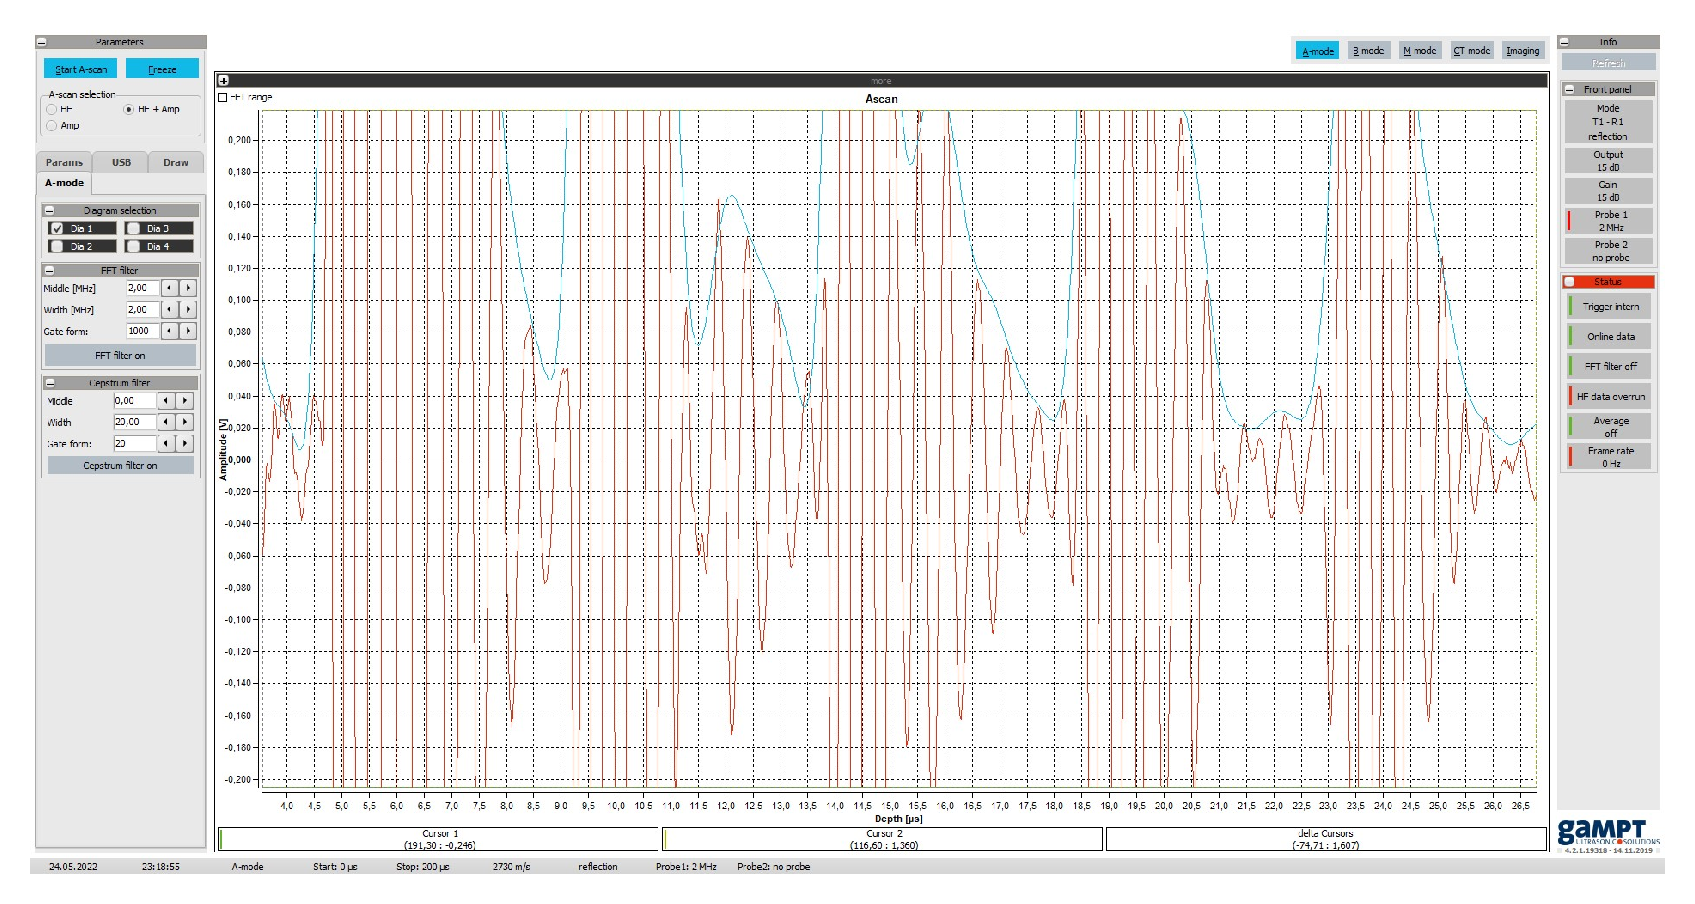
\includegraphics[width =\linewidth]{pictures/Schallgeschwindigkeit/Messung1.pdf}
  \caption{Screenshot der Messung der Acrylplatte.}
  \label{fig:messung1}
\end{figure}

Weiterhin soll die Frequenz bestimmt werden.
Dies geschieht über das Abschätzen der Periodenlänge.
Dafür werden 5 Periodenlängen aus \autoref{fig:messung2} abgelesen und gemittelt.
Daraus ergibt sich dann
\begin{equation*}
  \increment T = \frac{2.3 \, \unit{\micro\second}}{5} = 0.46 \, \unit{\micro\second},
\end{equation*}
woraus sich
\begin{align*}
  f = \frac{1}{T} = 2.174 \, \unit{\mega\hertz} && \text{und} && \lambda = \frac{c}{f} = (1.26 \pm 0.12) \cdot 10^{-3} \, \unit\meter\\
\end{align*}
ergeben.
Die Tiefenmessung des Programms ergibt dann eine Tiefe von $d = 0.6 \, \unit{\centi\meter}$.


\begin{figure} [H]
  \centering
  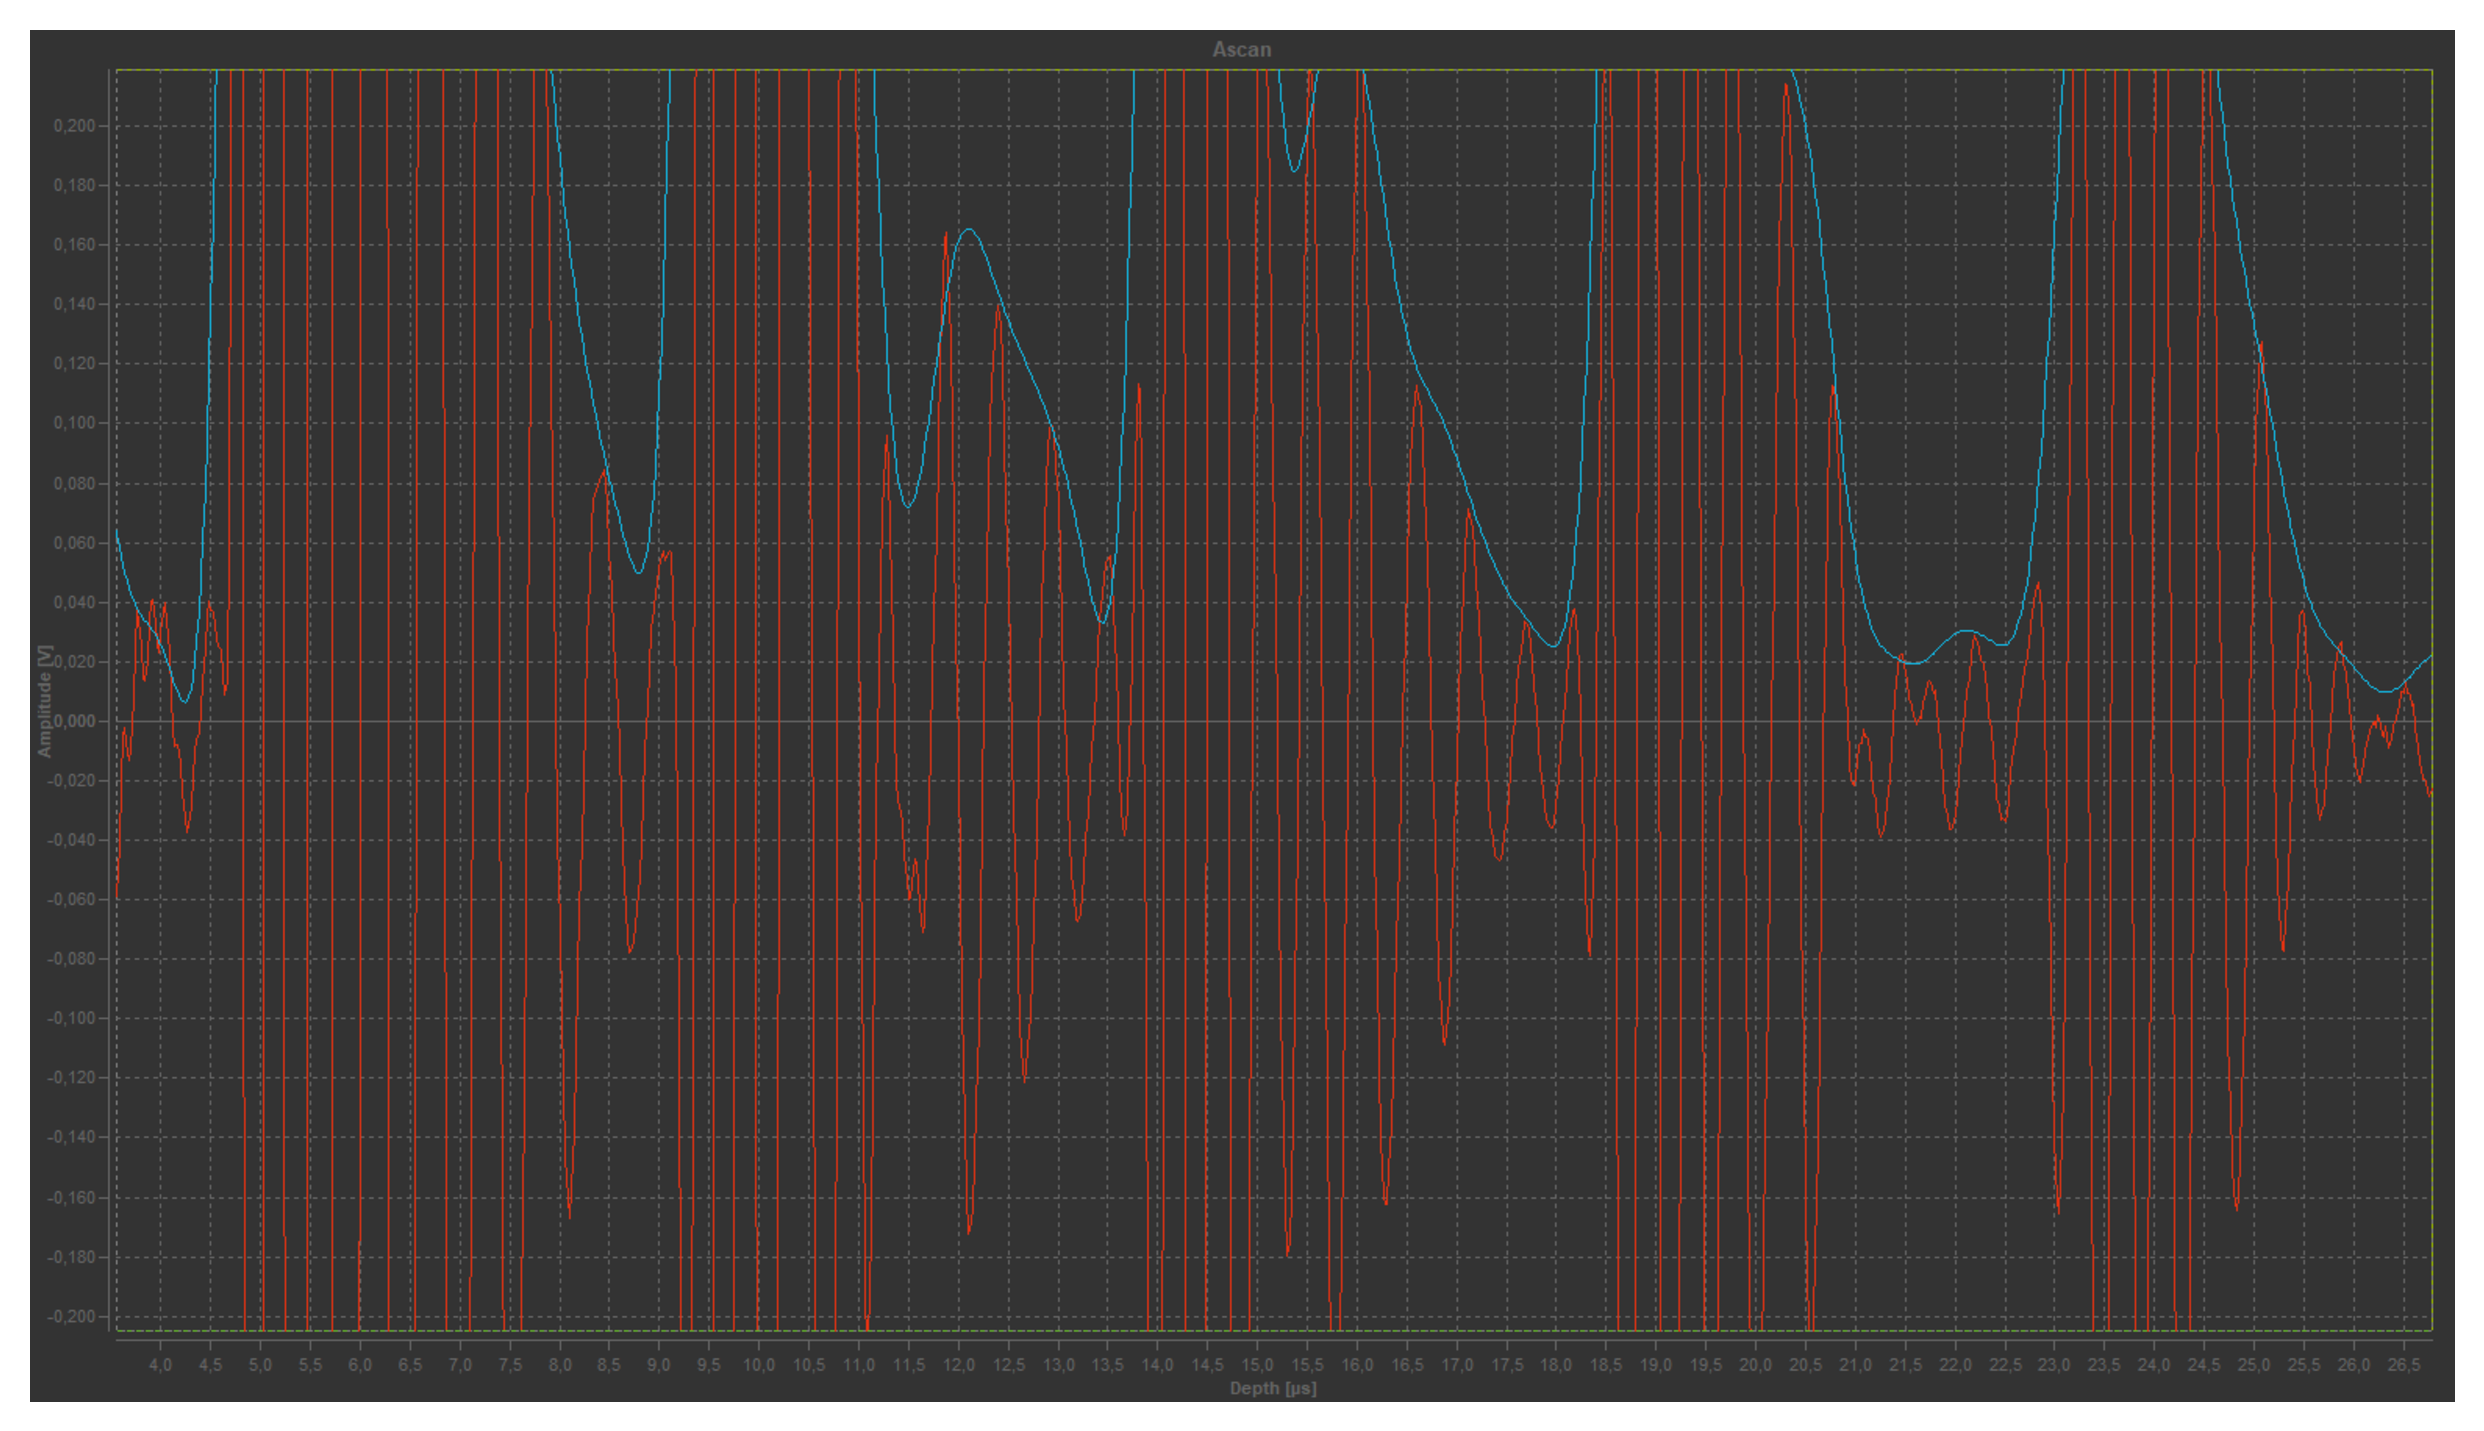
\includegraphics[width =\linewidth]{pictures/Schallgeschwindigkeit/Messung2.pdf}
  \caption{Screenshot der Messung der Acrylplatte im anderen Modus.}
  \label{fig:messung2}
\end{figure}


\subsection{Bestimmung der Schallgeschwindigkeit mit dem Impuls-Echo-Verfahren}

Die Messungen sind in \autoref{fig:echo_messungen} zu finden.
Die daraus entnommenen Messdaten sind in \autoref{tab:echo_messungen} zu finden.
Dabei ist für die Kombination $1 + 3$, dargestellt in \autoref{fig:echo_z1_z3} kein Peak für die entsprechende Länge zu erkennen.
Die zu sehenden Peaks sind jeweils den einzelnen Zylindern zuzuordnen, nicht der Kombination der beiden.
Deshalb muss diese Messung im folgenden verworfen werden.
Um die Schallgeschwindigkeit zu bestimmen, wird der Ansatz
\begin{equation*}
  2 \cdot d = t \cdot c + b
\end{equation*}
gemacht. Die lineare Regression ist in \autoref{fig:plot1} zu finden.
Der Ansatz ergibt die Werte
\begin{align*}
  c = (2740 \pm 10)  \, \unit{\meter / \second} \quad \text{und} \quad
  b = -(2.4 \pm 0.8) \cdot 10^{-3} \, \unit{\meter / \second} \, .
\end{align*}

\begin{figure}
  \centering
  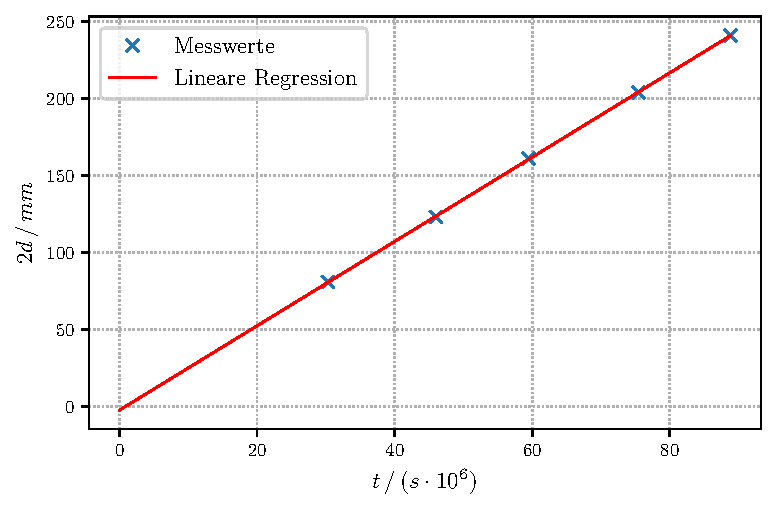
\includegraphics[width = 0.7\linewidth]{build/plot1.pdf}
  \caption{Regressionsgerade der Messdaten des Impuls-Echo-Verfahrens.}
  \label{fig:plot1}
\end{figure}

\begin{table}
  \centering
  \caption{Messdaten des Impuls-Echo-Verfahrens.}
  \label{tab:echo_messungen}
  \begin{tabular}{c | c c c c}
      \toprule
      Zylinder& Höhe / $\unit\meter$ & t / \unit{\micro\second} & $U_0$ & $U_t$\\ 
      \midrule
      1     & 0.0404 & 30.3 & 1.31 & 0.92 \\
      2     & 0.0615 & 46.0 & 1.31 & 0.25 \\
      3     & 0.0805 & 59.5 & 1.31 & 0.11 \\
      1 + 2 & 0.1019 & 75.5 & 1.31 & 0.2  \\
      1 + 3 & 0.1209 &  -   & 1.31 & -    \\
      4     & 0.1205 & 88.8 & 1.31 & 0.012\\
      \bottomrule
  \end{tabular}
\end{table}

\begin{figure}%
  \begin{subfigure}{0.48\textwidth}%
  \centering%
  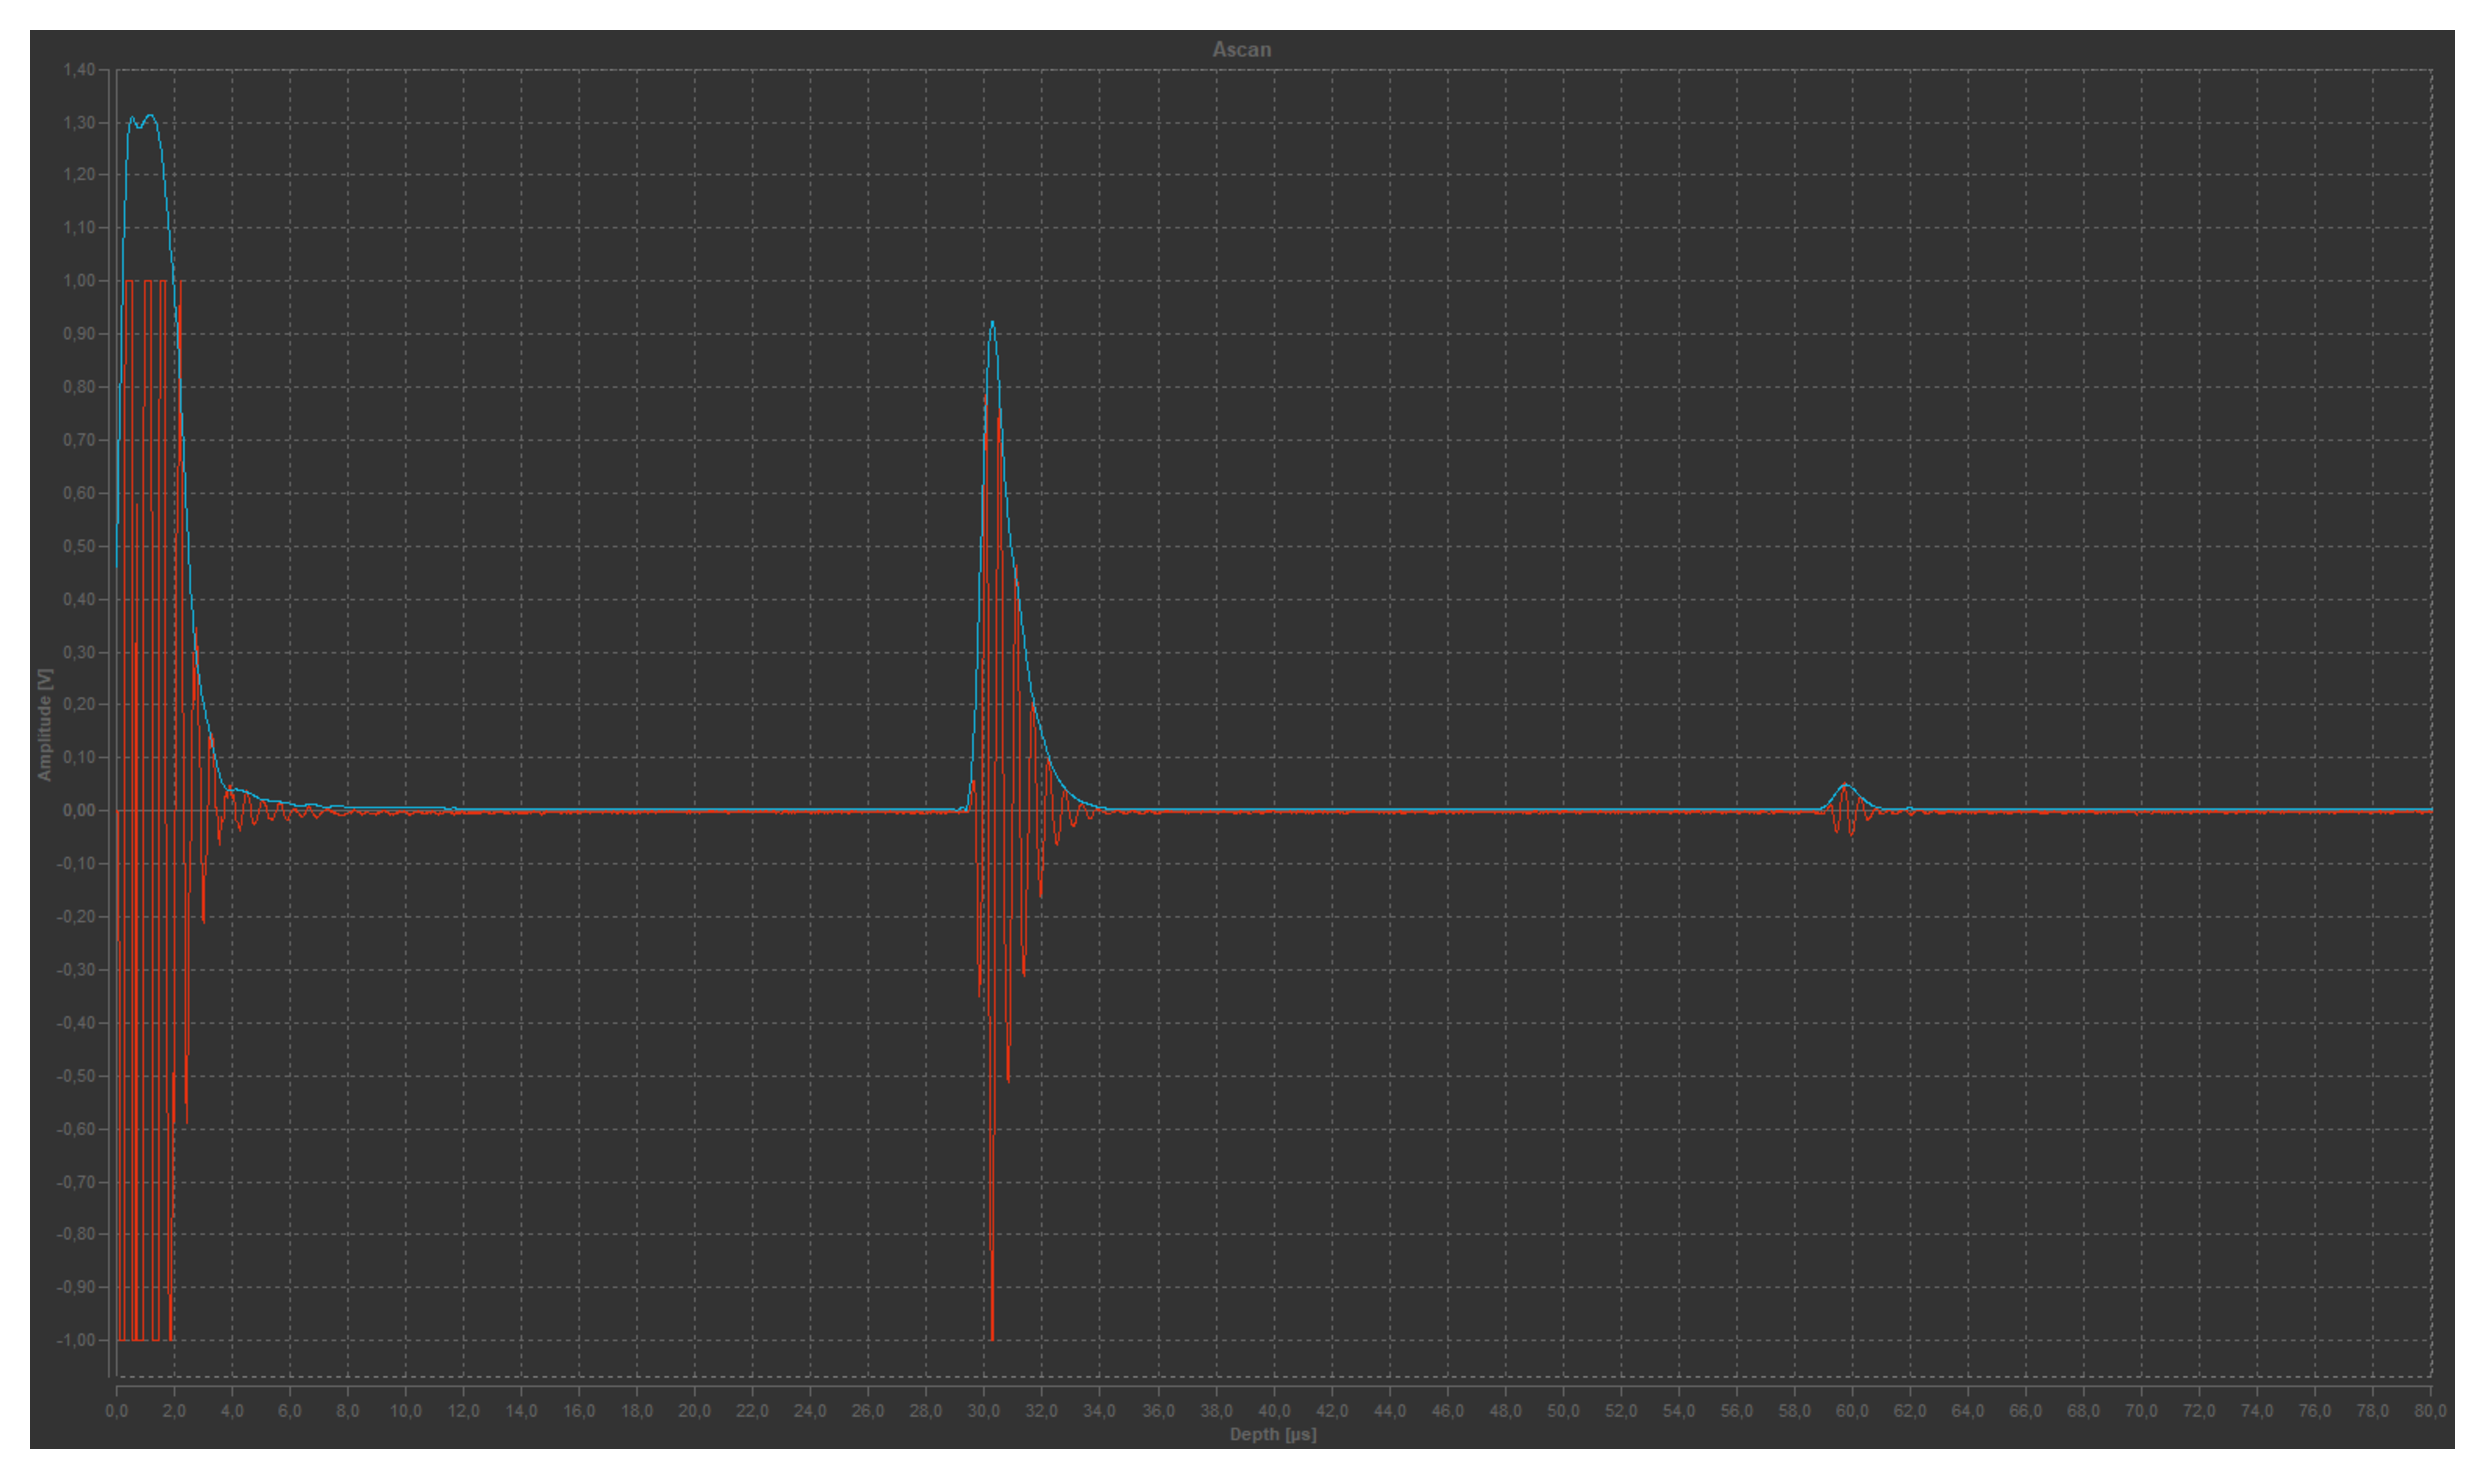
\includegraphics[width=\linewidth]{pictures/Impuls-Echo-Zylinder/z1.pdf}%
  \caption{Der erste Zylinder.}%
  \label{fig:echo_z1}%
  \end{subfigure}%
  \hfill%
  \begin{subfigure}{0.48\textwidth}%
  \centering%
  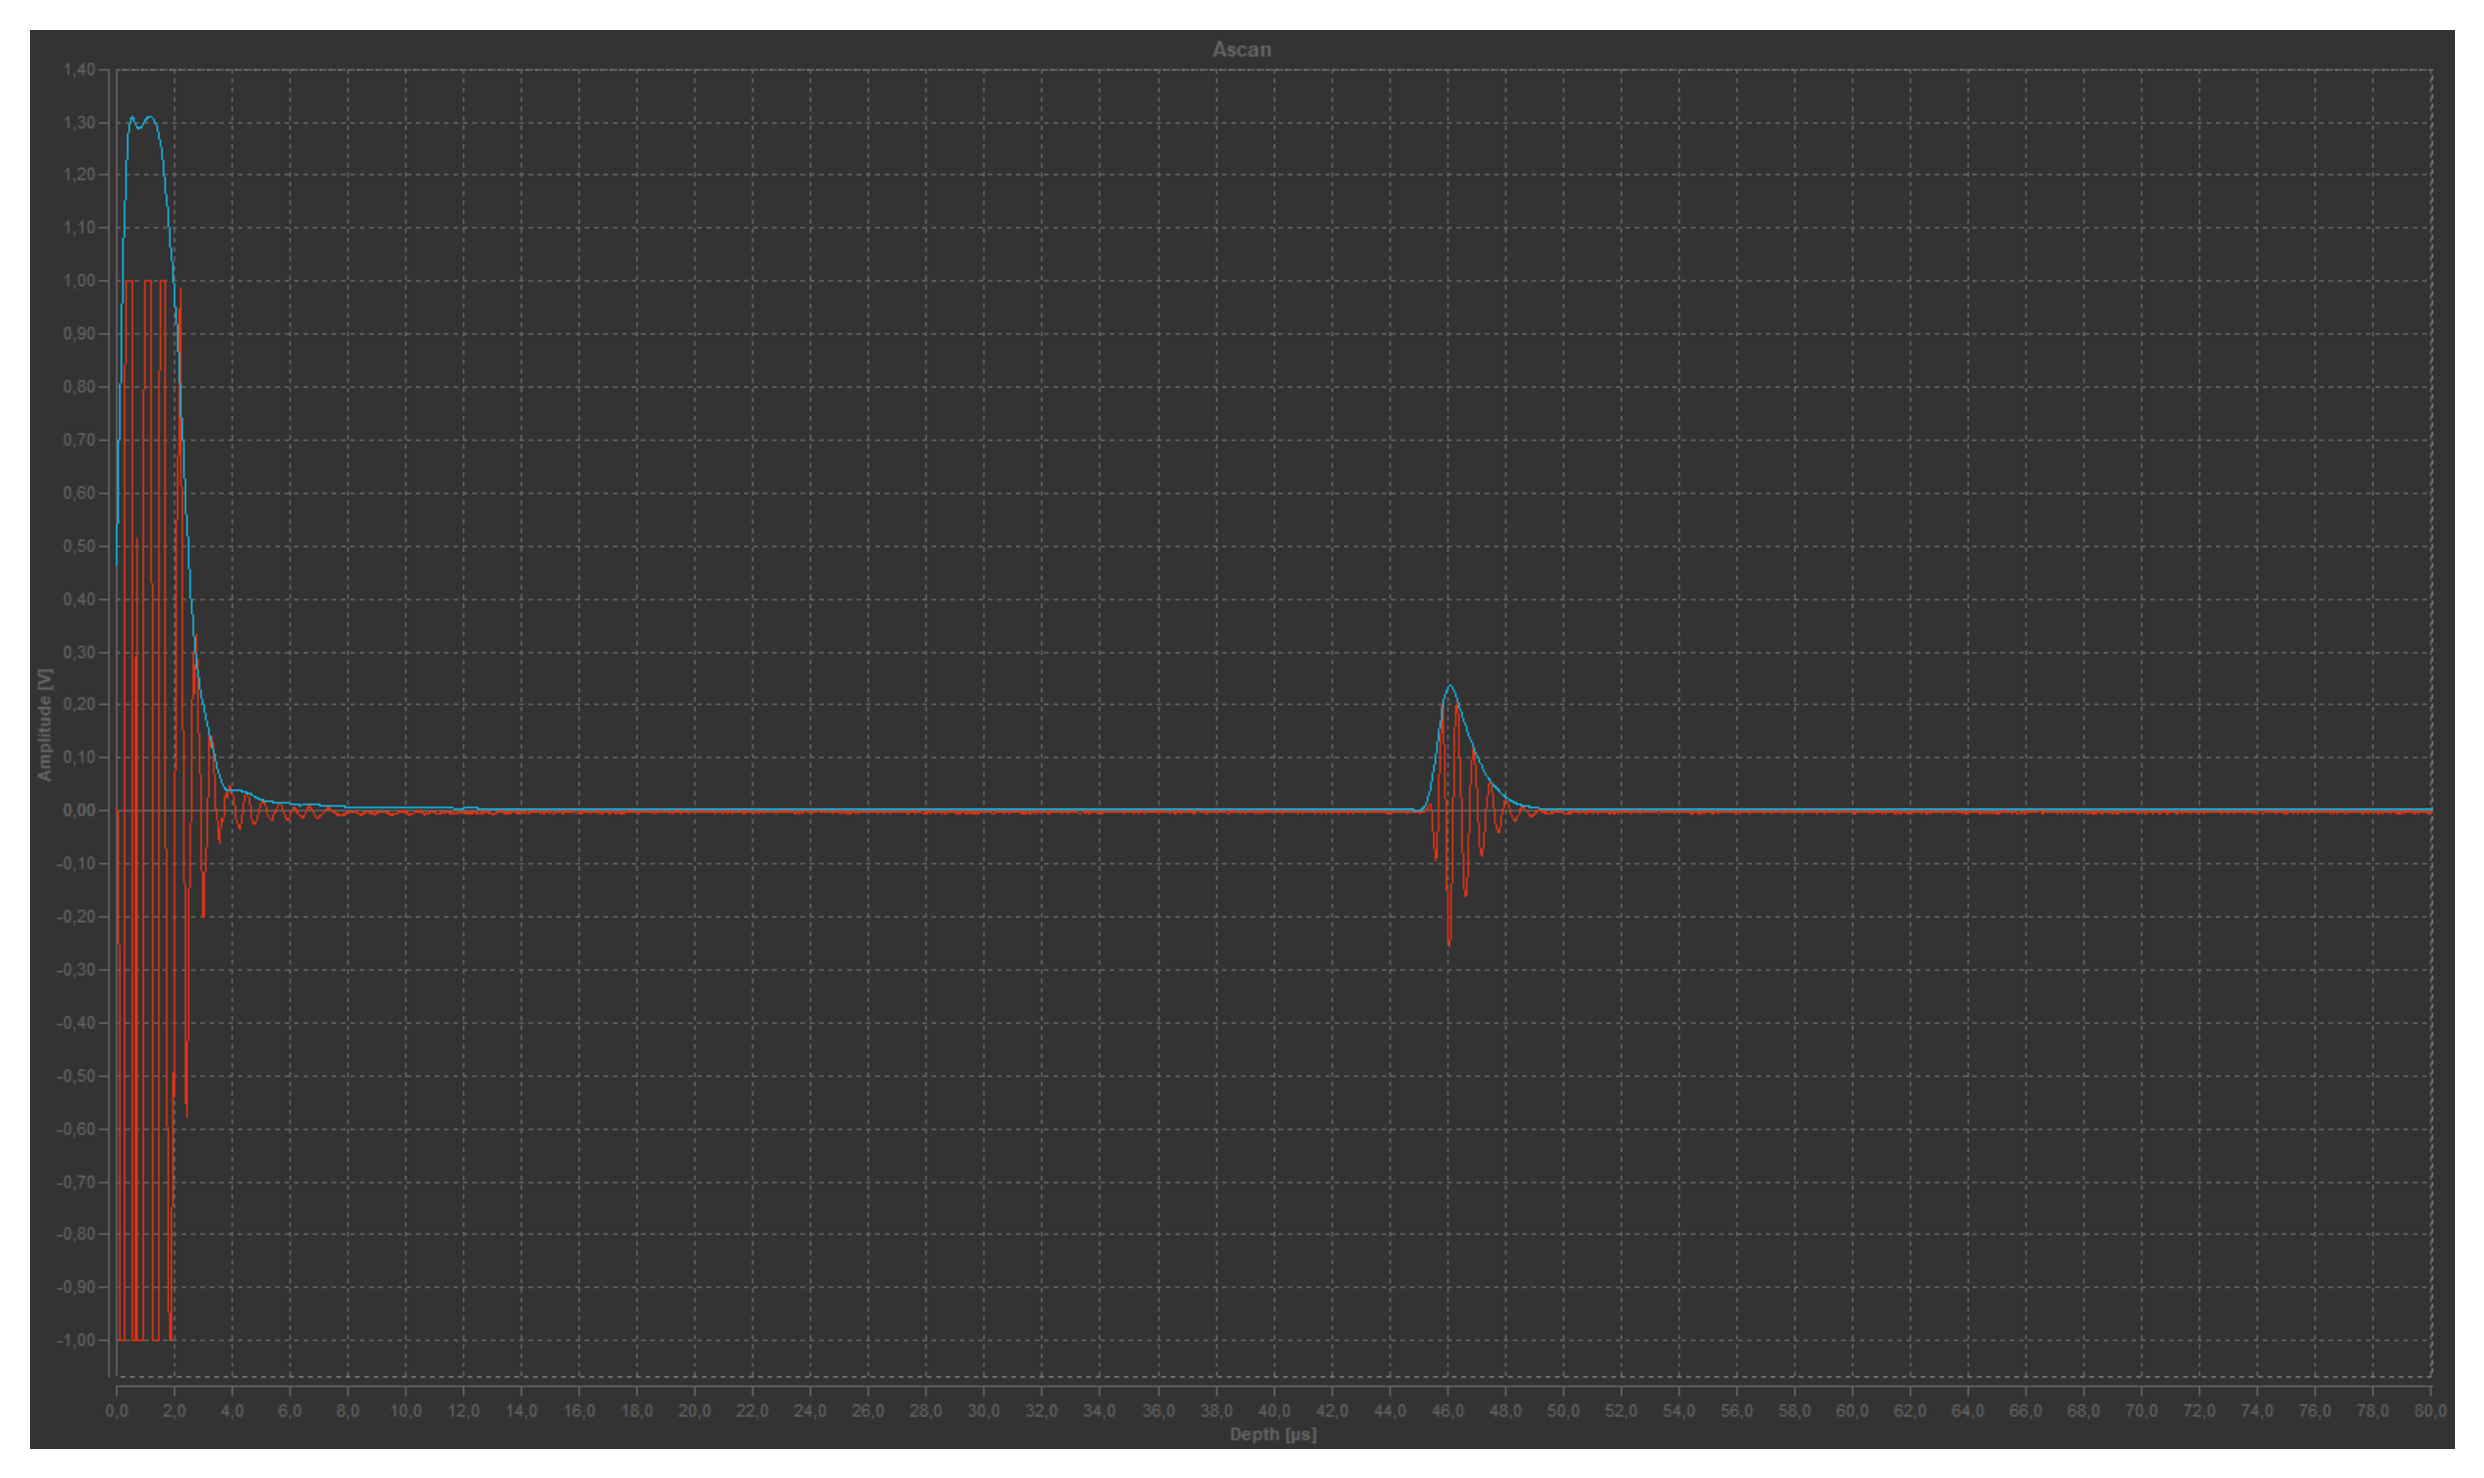
\includegraphics[width=\linewidth]{pictures/Impuls-Echo-Zylinder/z2.pdf}%
  \caption{Der zweite Zylinder.}%
  \label{fig:echo_z2}%
  \end{subfigure}%
  \hfill

  \begin{subfigure}{0.48\textwidth}%
  \centering%
  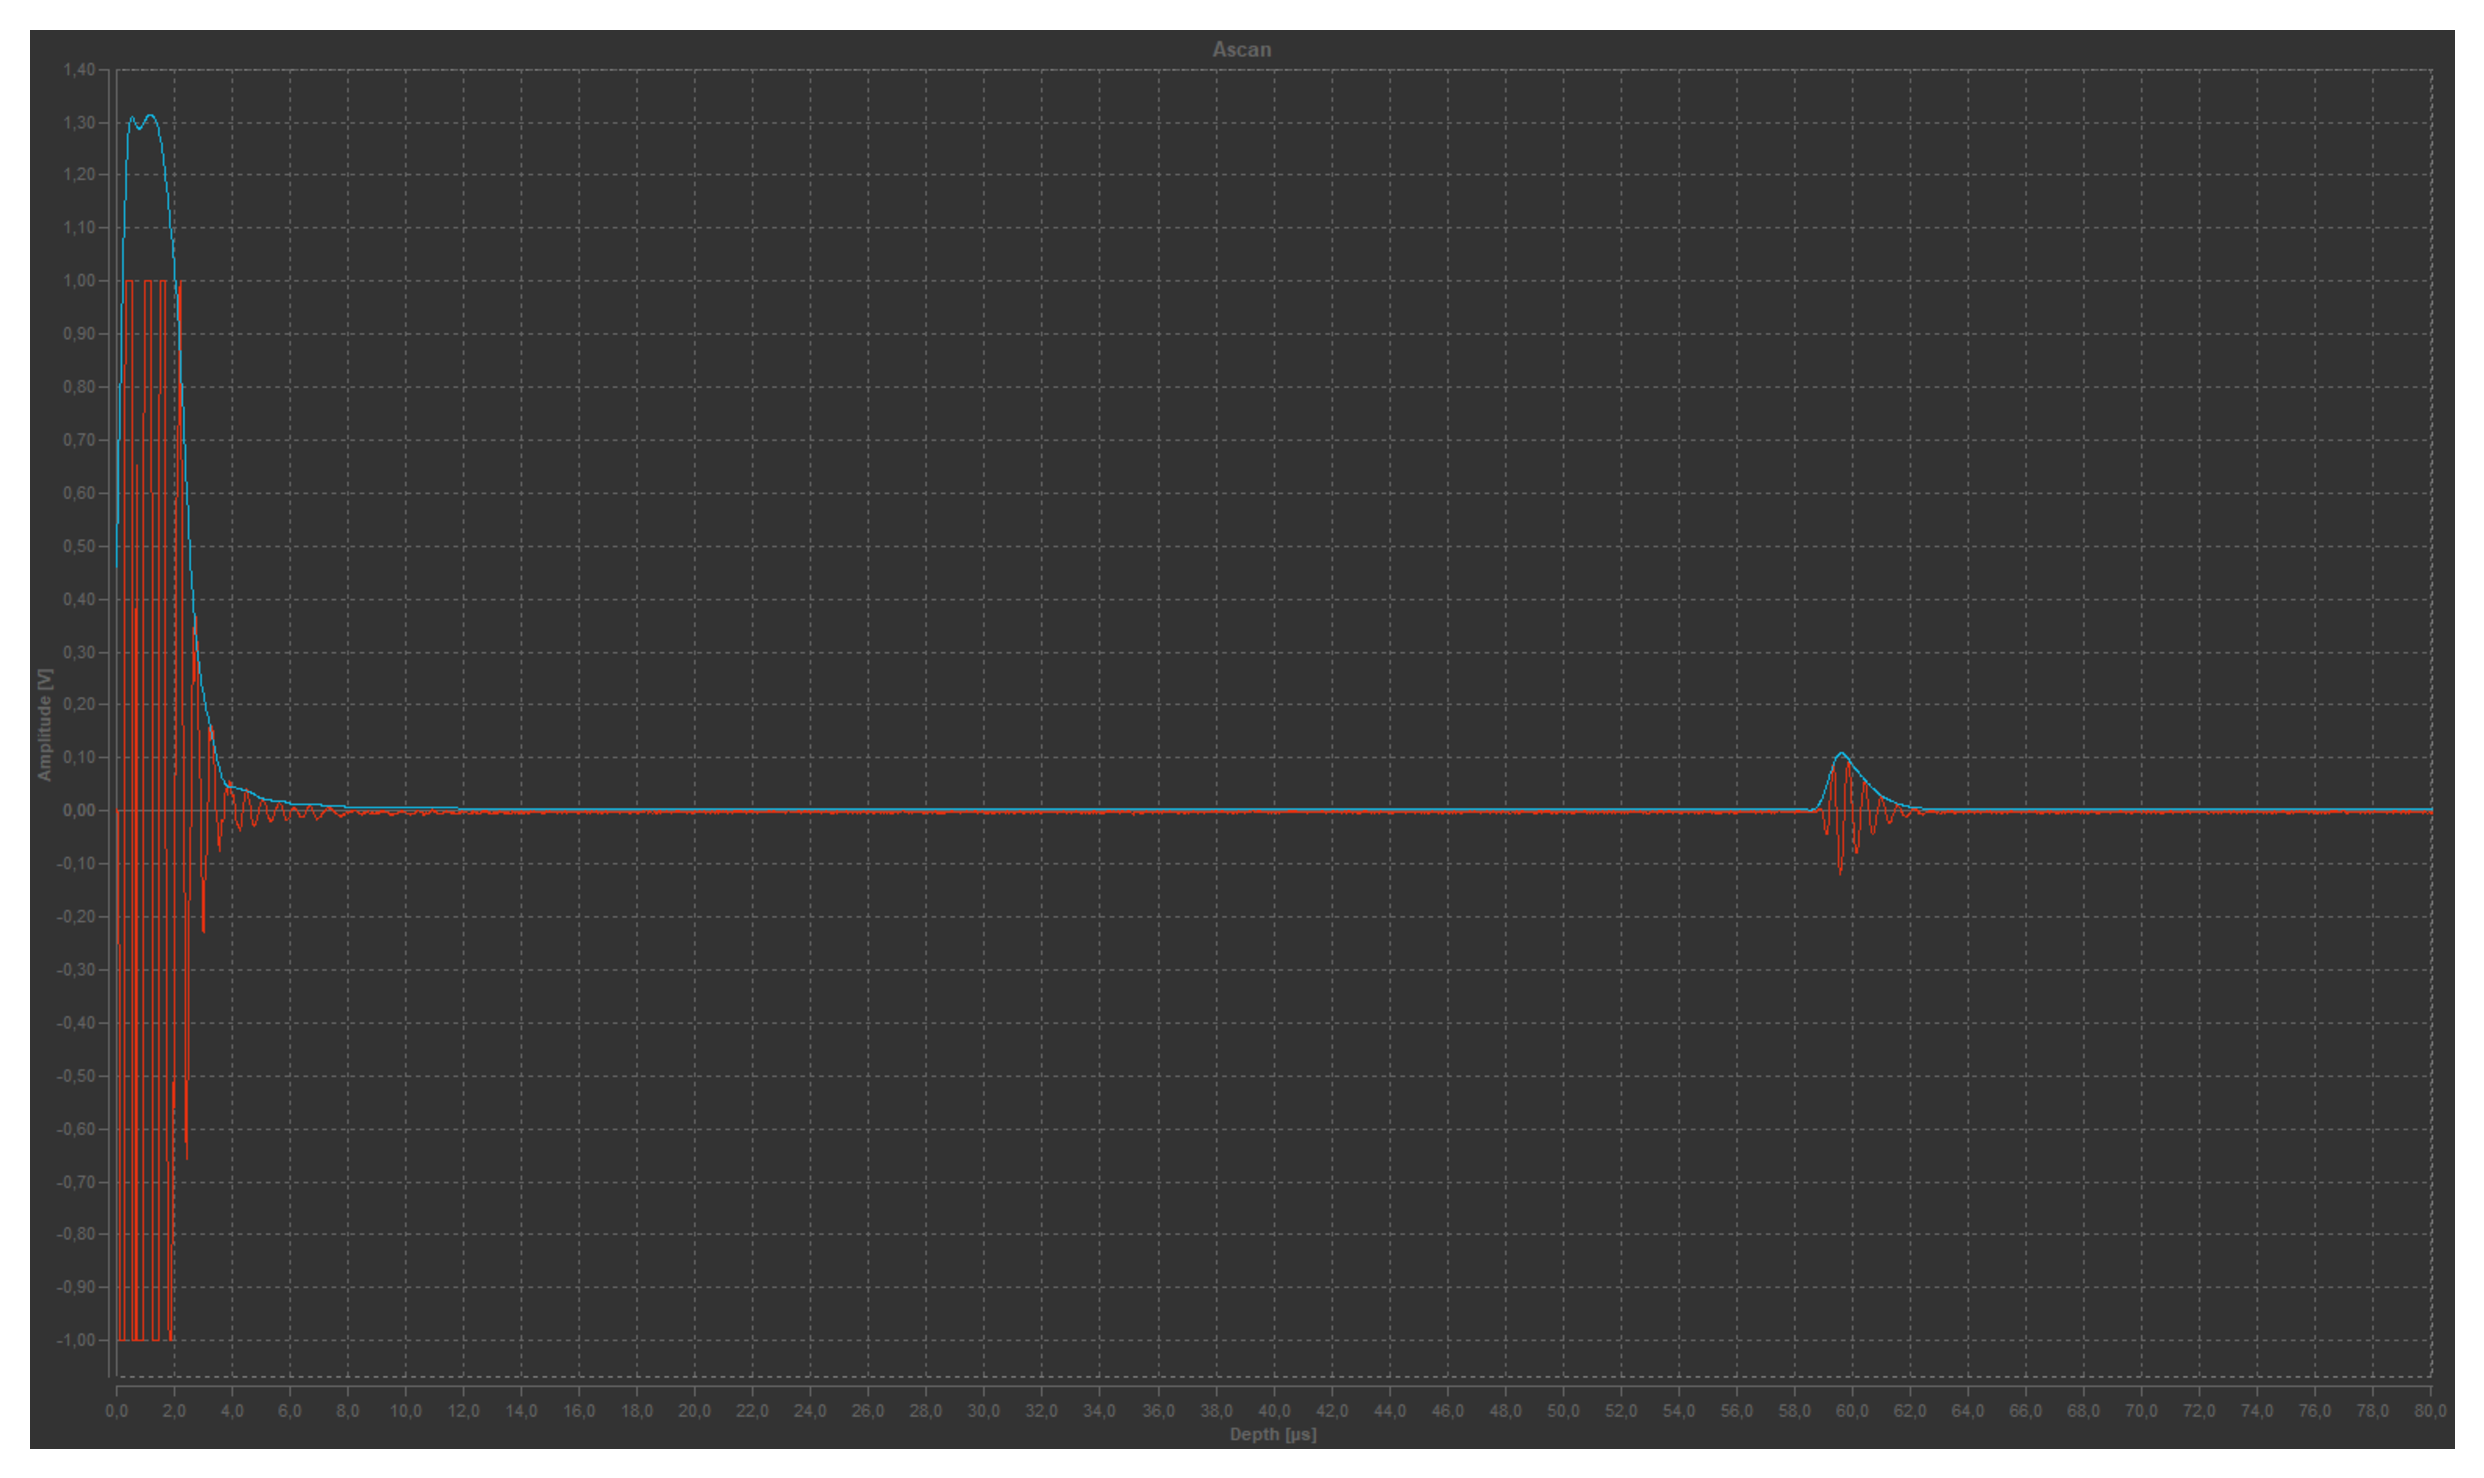
\includegraphics[width=\linewidth]{pictures/Impuls-Echo-Zylinder/z3.pdf}%
  \caption{Der dritte Zylinder.}%
  \label{fig:echo_z3}%
  \end{subfigure}%
  \hfill%
  \begin{subfigure}{0.48\textwidth}%
  \centering%
  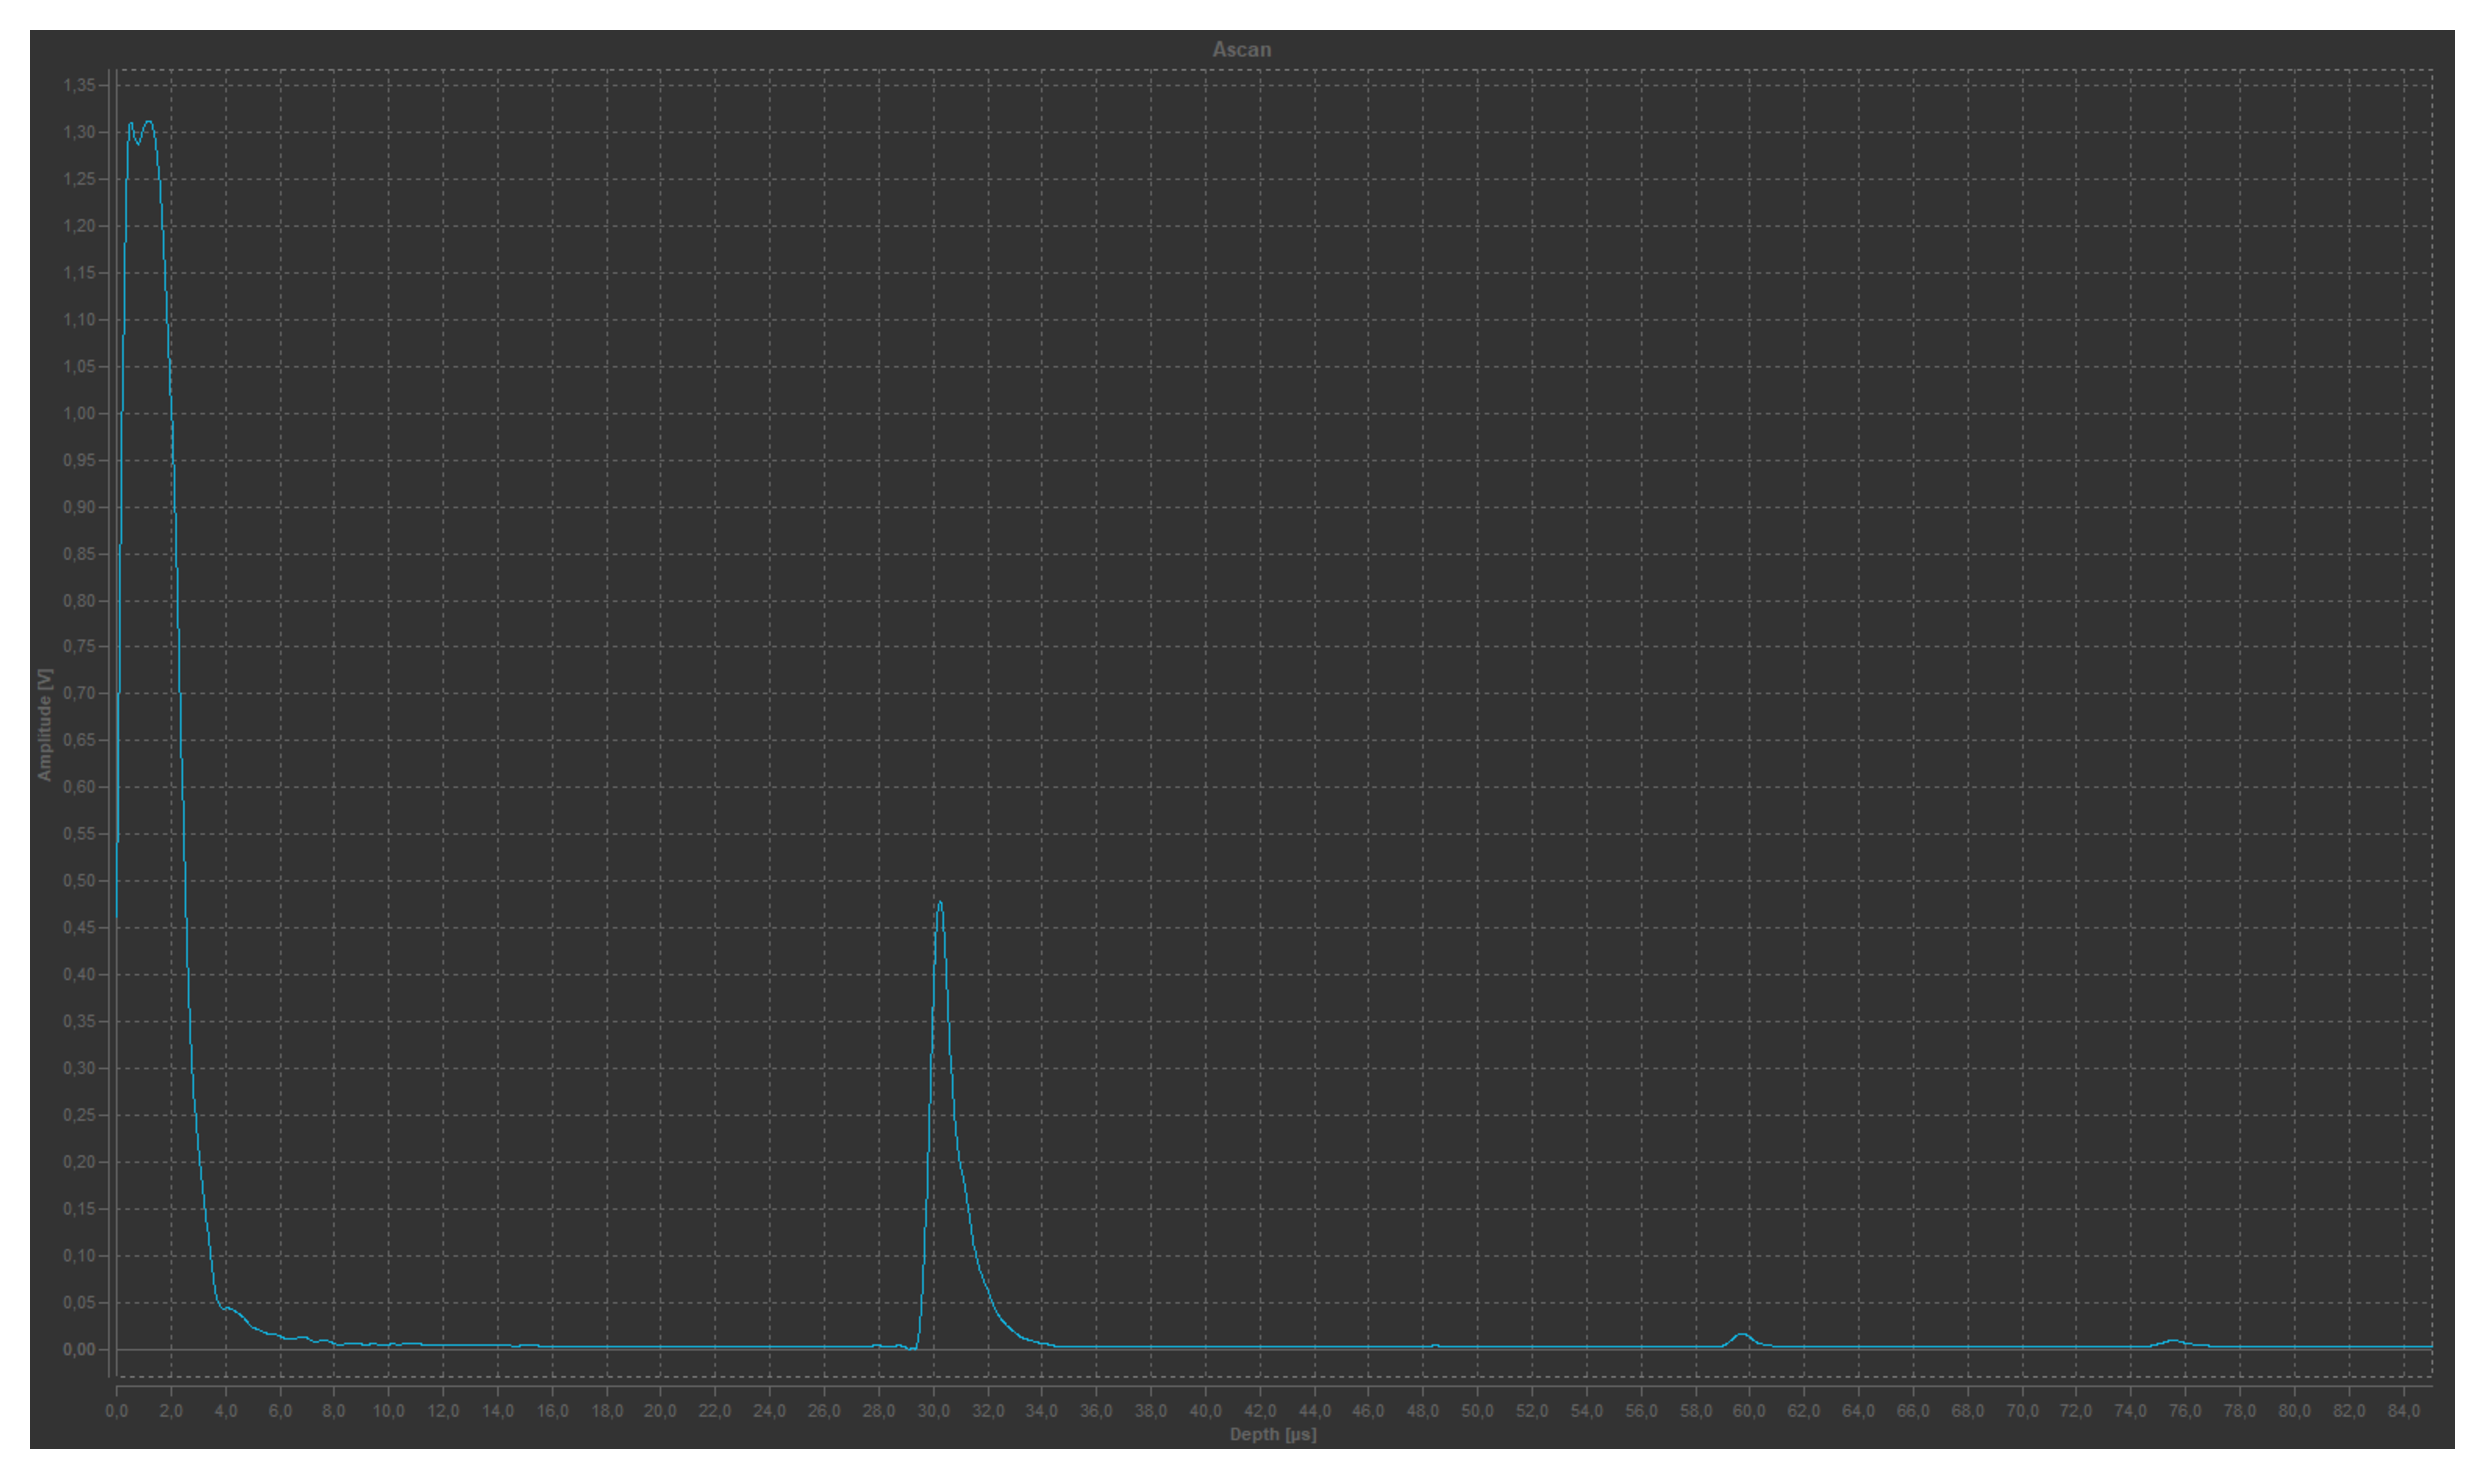
\includegraphics[width=\linewidth]{pictures/Impuls-Echo-Zylinder/z1_z2.pdf}%
  \caption{Der erste und zweite Zylinder zusammen.}%
  \label{fig:echo_z1_z2}%
  \end{subfigure}%
  \hfill

  \begin{subfigure}{0.48\textwidth}%
  \centering%
  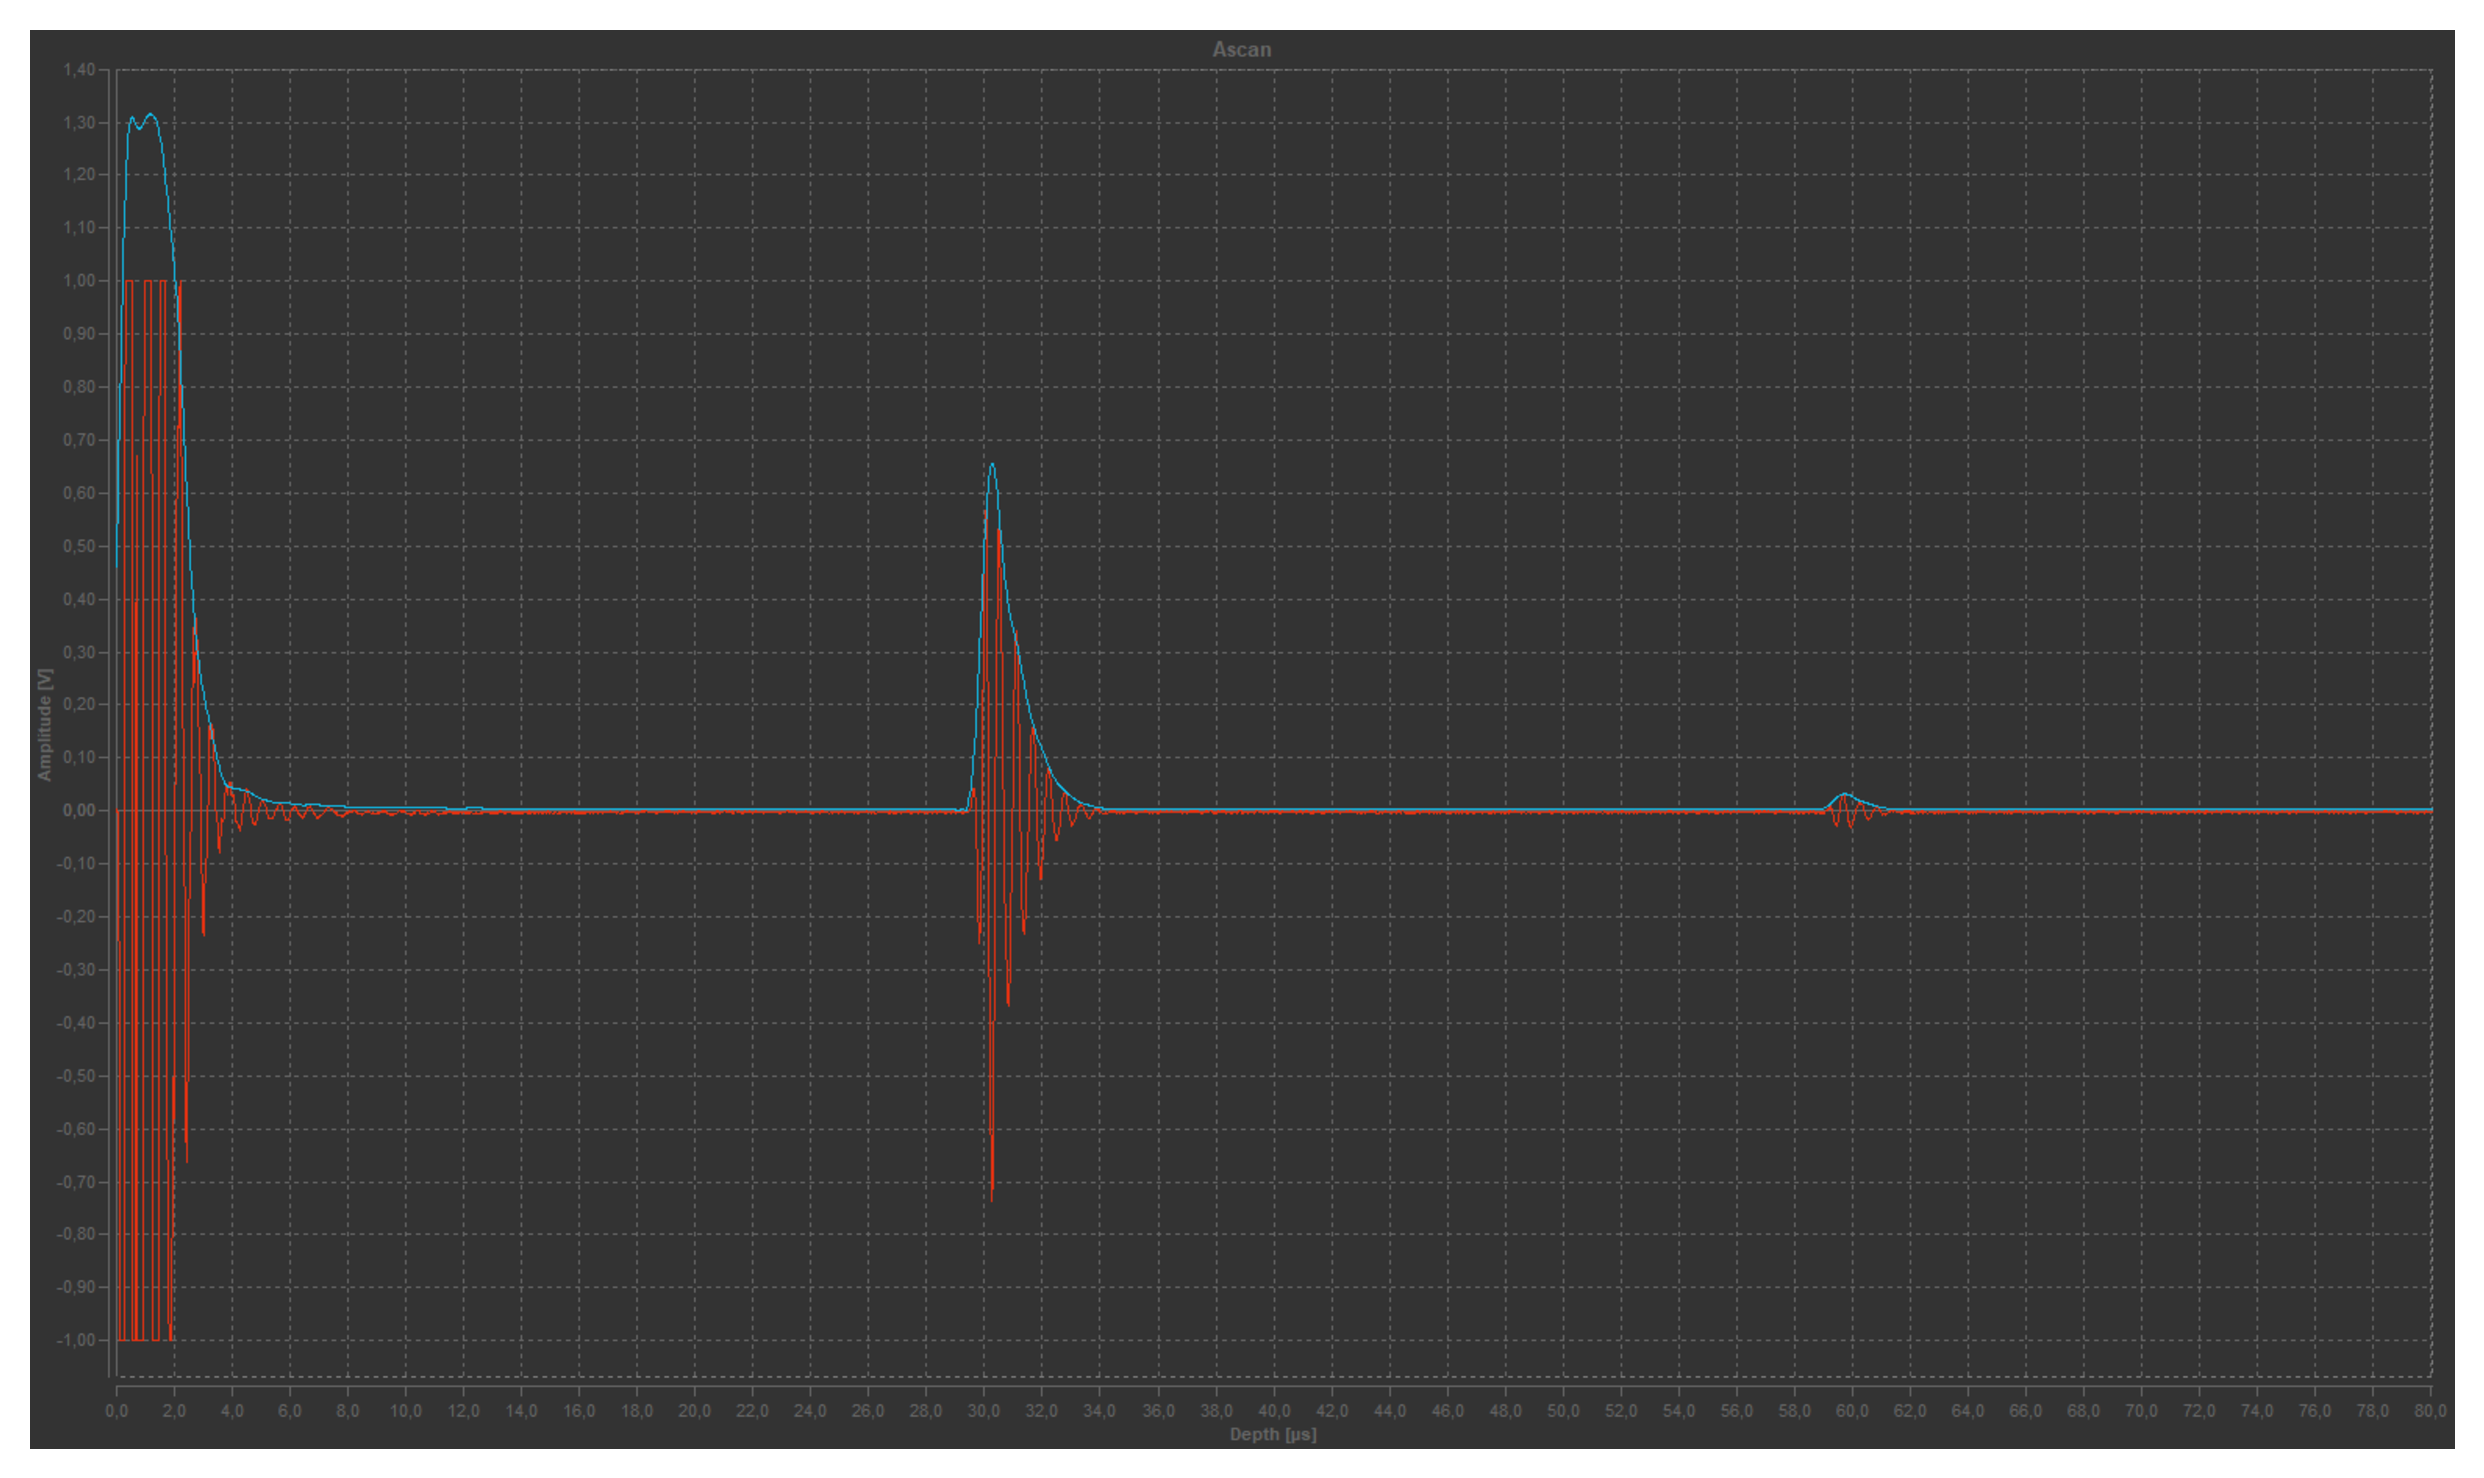
\includegraphics[width=\linewidth]{pictures/Impuls-Echo-Zylinder/z1_z3.pdf}%
  \caption{Der erste und der dritte Zylinder zusammen.}%
  \label{fig:echo_z1_z3}%
  \end{subfigure}%
  \hfill%
  \begin{subfigure}{0.48\textwidth}%
  \centering%
  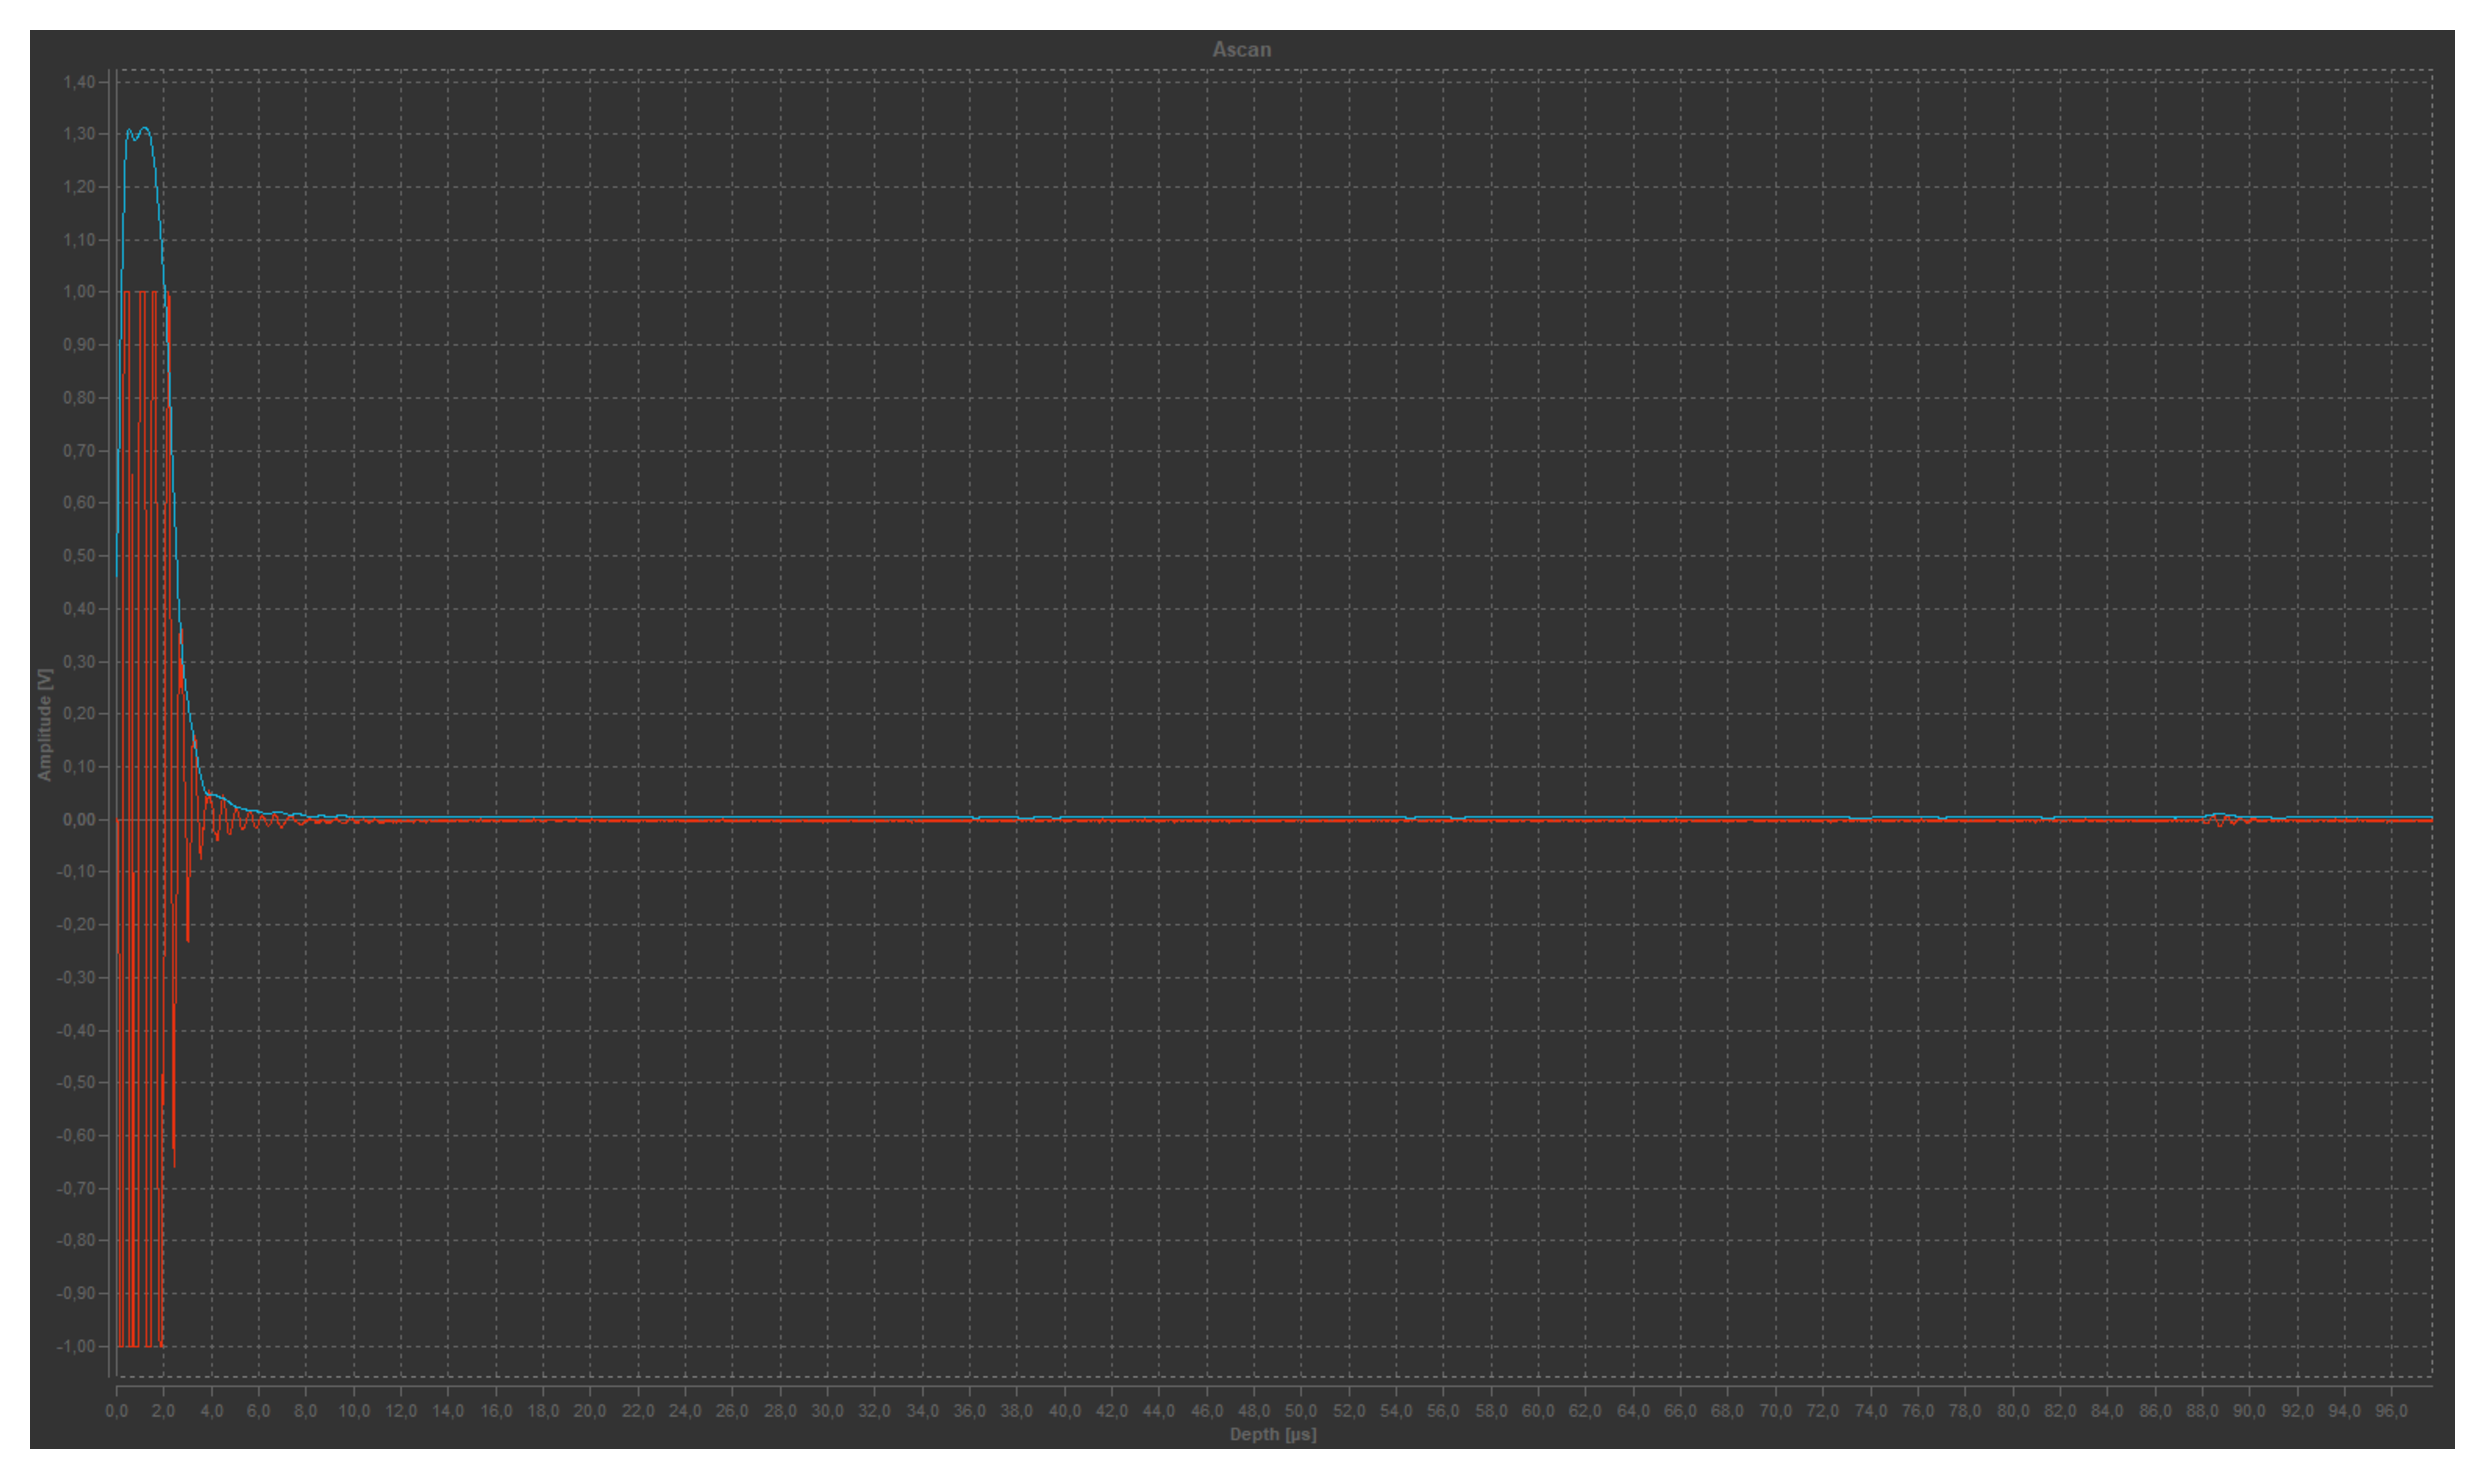
\includegraphics[width=\linewidth]{pictures/Impuls-Echo-Zylinder/z4_(1).pdf}%
  \caption{Der vierte Zylinder.}%
  \label{fig:echo_z4_(1)}%
  \end{subfigure}%
  \hfill

  \begin{subfigure}{\textwidth}%
  \centering%
  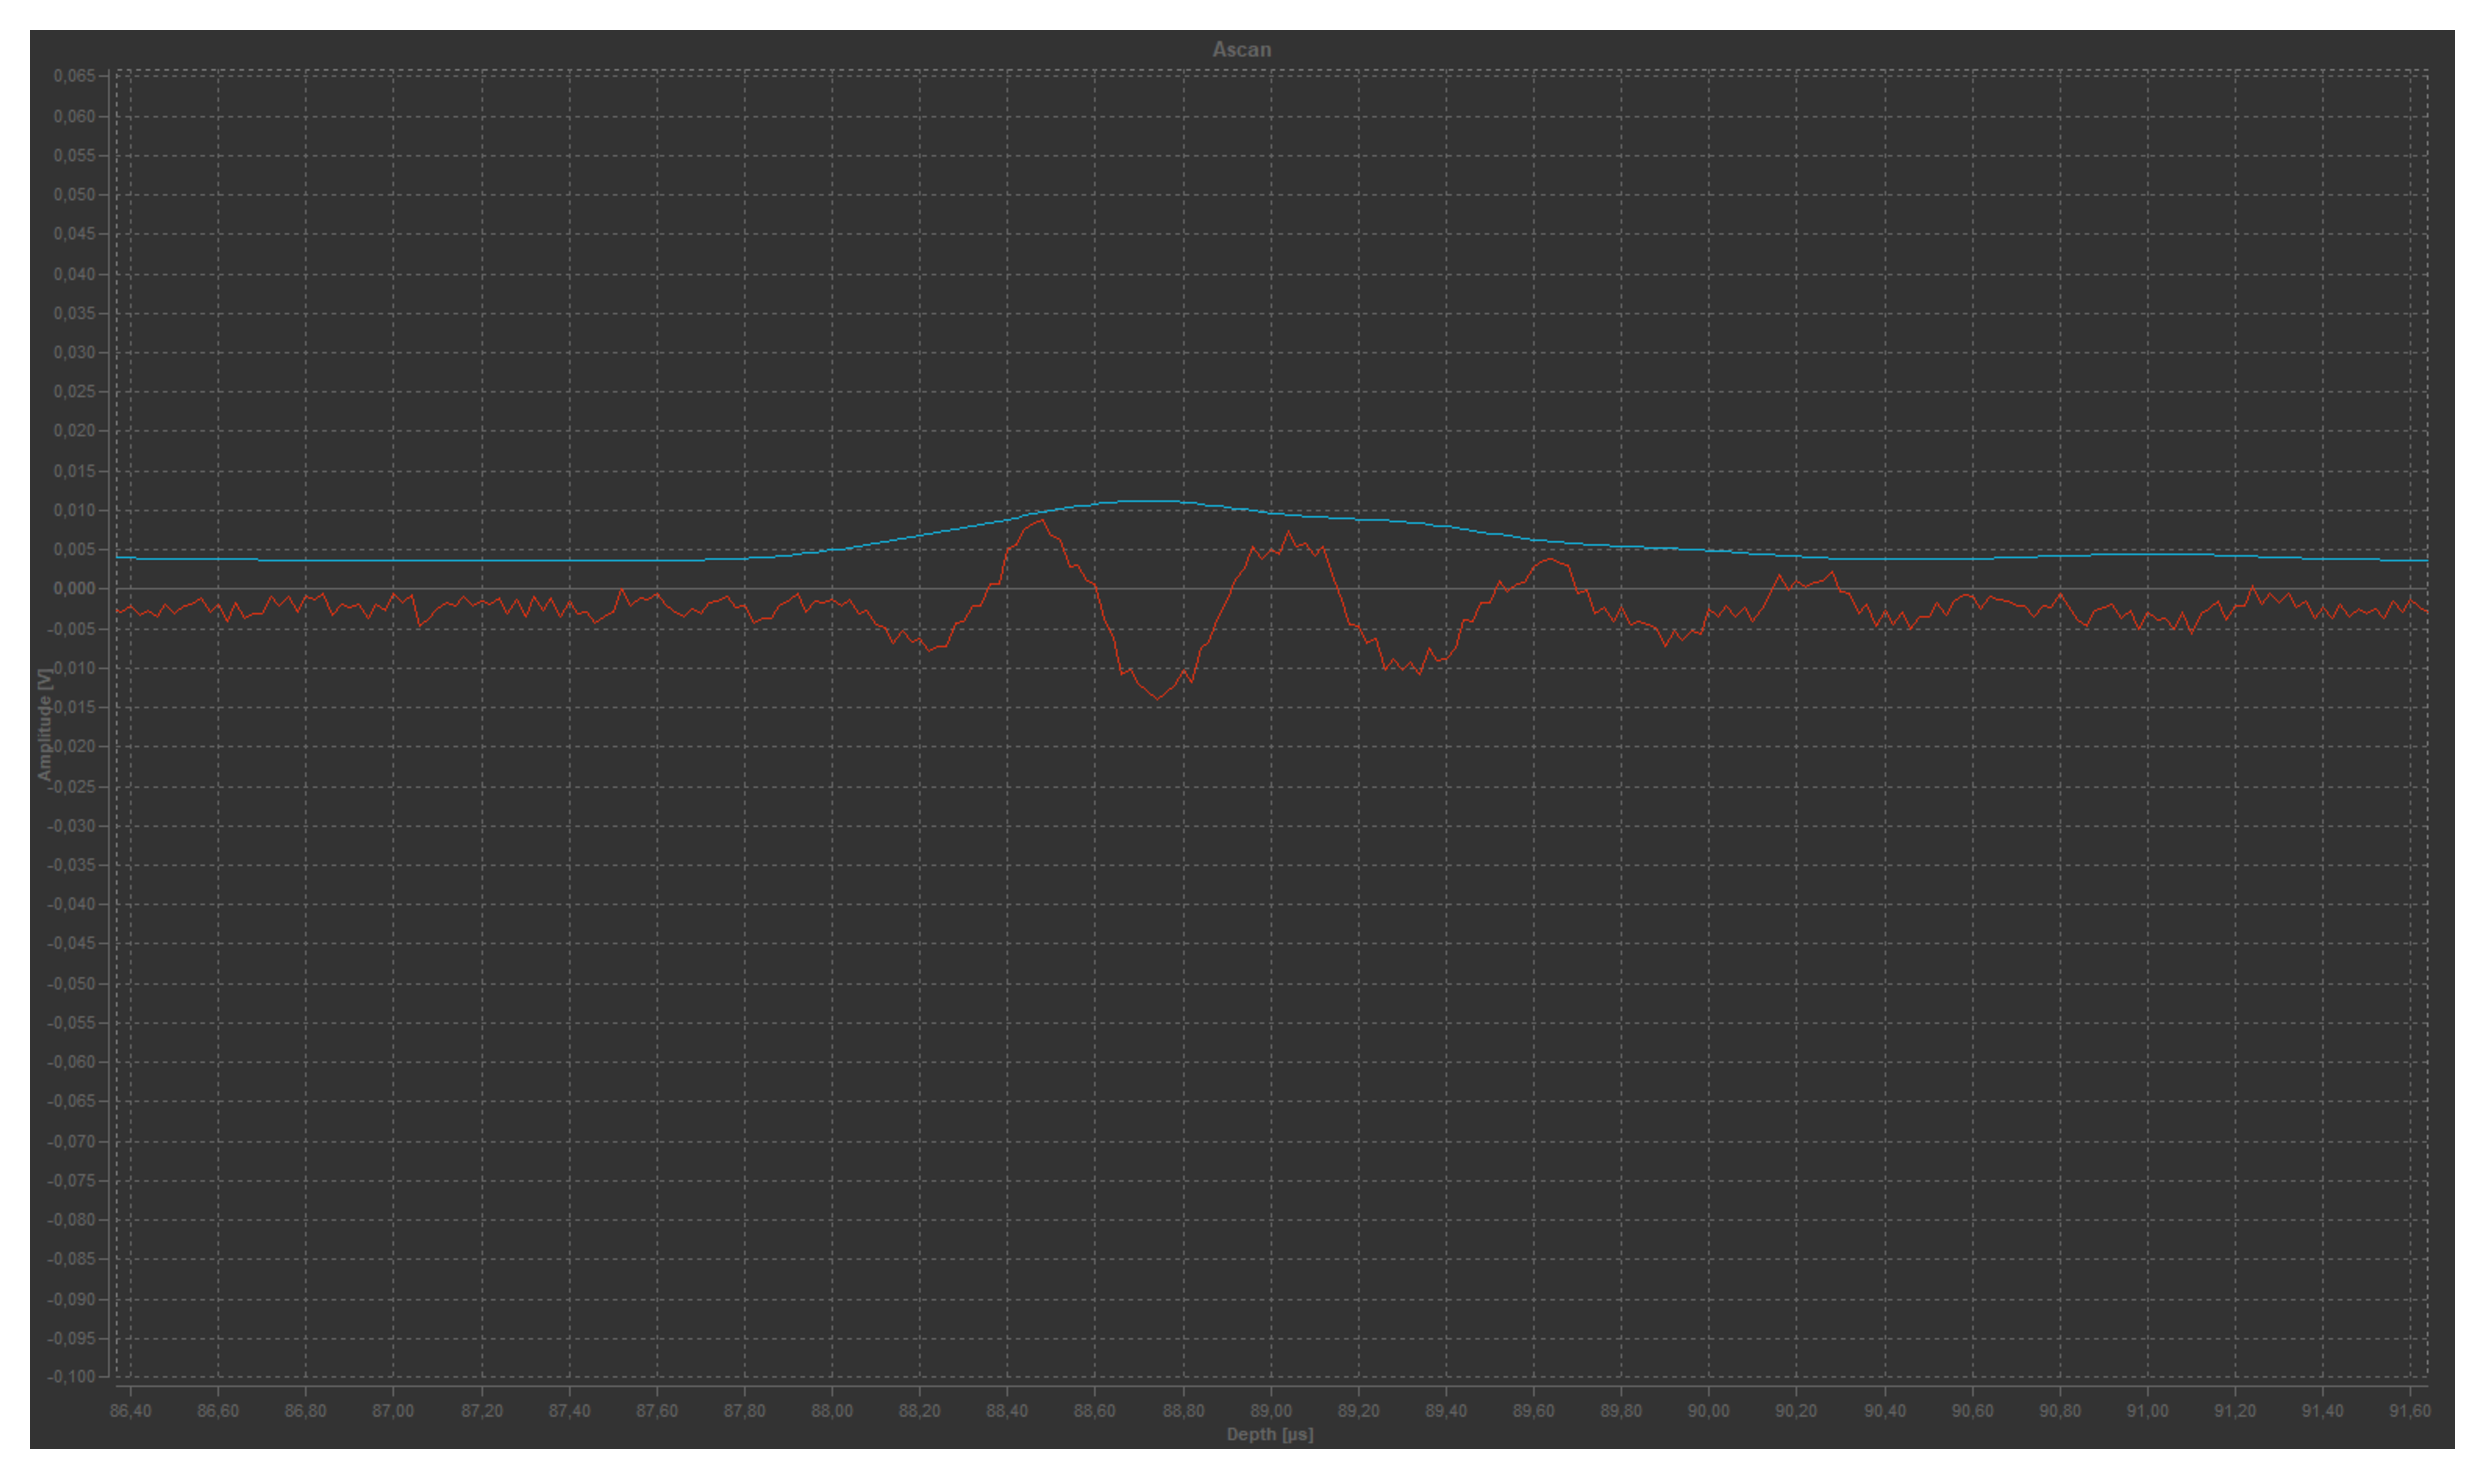
\includegraphics[width=0.48 \linewidth]{pictures/Impuls-Echo-Zylinder/z4_(2).pdf}%
  \caption{Der zweite Peak des vierten Zylinders in naher Aufnahme.}%
  \label{fig:echo_z4_(2)}%
  \end{subfigure}%
  \caption{Die Messungen des Impuls-Echo-Verfahrens}%
  \label{fig:echo_messungen}%
\end{figure}%


\subsection{Bestimmung der Schallgeschwindigkeit mit dem Durchschallungs-Verfahren}

Da bei diesem Verfahren der Schall den jeweiligen Körper nur einmal durchläuft, ergibt sich als Ansatz für die Regression die Formel
\begin{equation*}
  d = t \cdot c + b \, .
\end{equation*}
Die Messungen werden in Screenshots gespeichert und sind in \autoref{fig:durchschallung_messungen} abgebildet.
Die Messwerte sind in \autoref{tab:durchschallung_messung} aufgetragen und die Regressionsgerade ist in \autoref{fig:plot2} abgebildet.
Aus dem Ansatz ergeben sich dann die Werte
\begin{align*}
  c = (2760 \pm 36)  \, \unit{\meter / \second} \quad \text{und} \quad b = -(4.21 \pm 1.11) \cdot 10^{-3} \, \unit{\meter / \second} \, .
\end{align*}

\begin{figure}
  \centering
  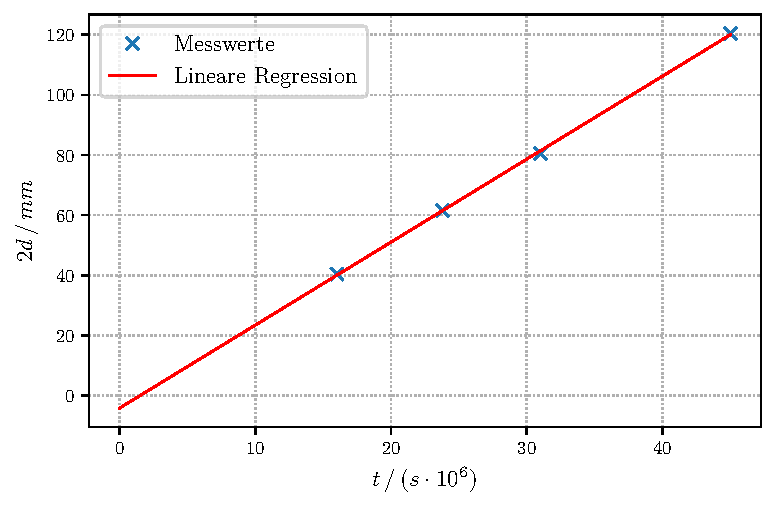
\includegraphics[width = 0.7\linewidth]{build/plot2.pdf}
  \caption{Regressionsgerade der Messdaten des Durchschallungs-Verfahrens.}
  \label{fig:plot2}
\end{figure}

\begin{table}
  \centering
  \caption{Messdaten des Durchschallungs-Verfahrens.}
  \label{tab:durchschallung_messung}
  \begin{tabular}{c | c c}
      \toprule
      Zylinder& Höhe / $\unit\meter$ & t / \unit{\micro\second}\\ 
      \midrule
      1     & 0.0404 & 16.0 \\
      2     & 0.0615 & 23.8 \\
      3     & 0.0805 & 31.0 \\
      4     & 0.1205 & 45.0 \\
      \bottomrule
  \end{tabular}
\end{table}

\begin{figure}[H]
  \begin{subfigure}{0.48\textwidth}%
  \centering%
  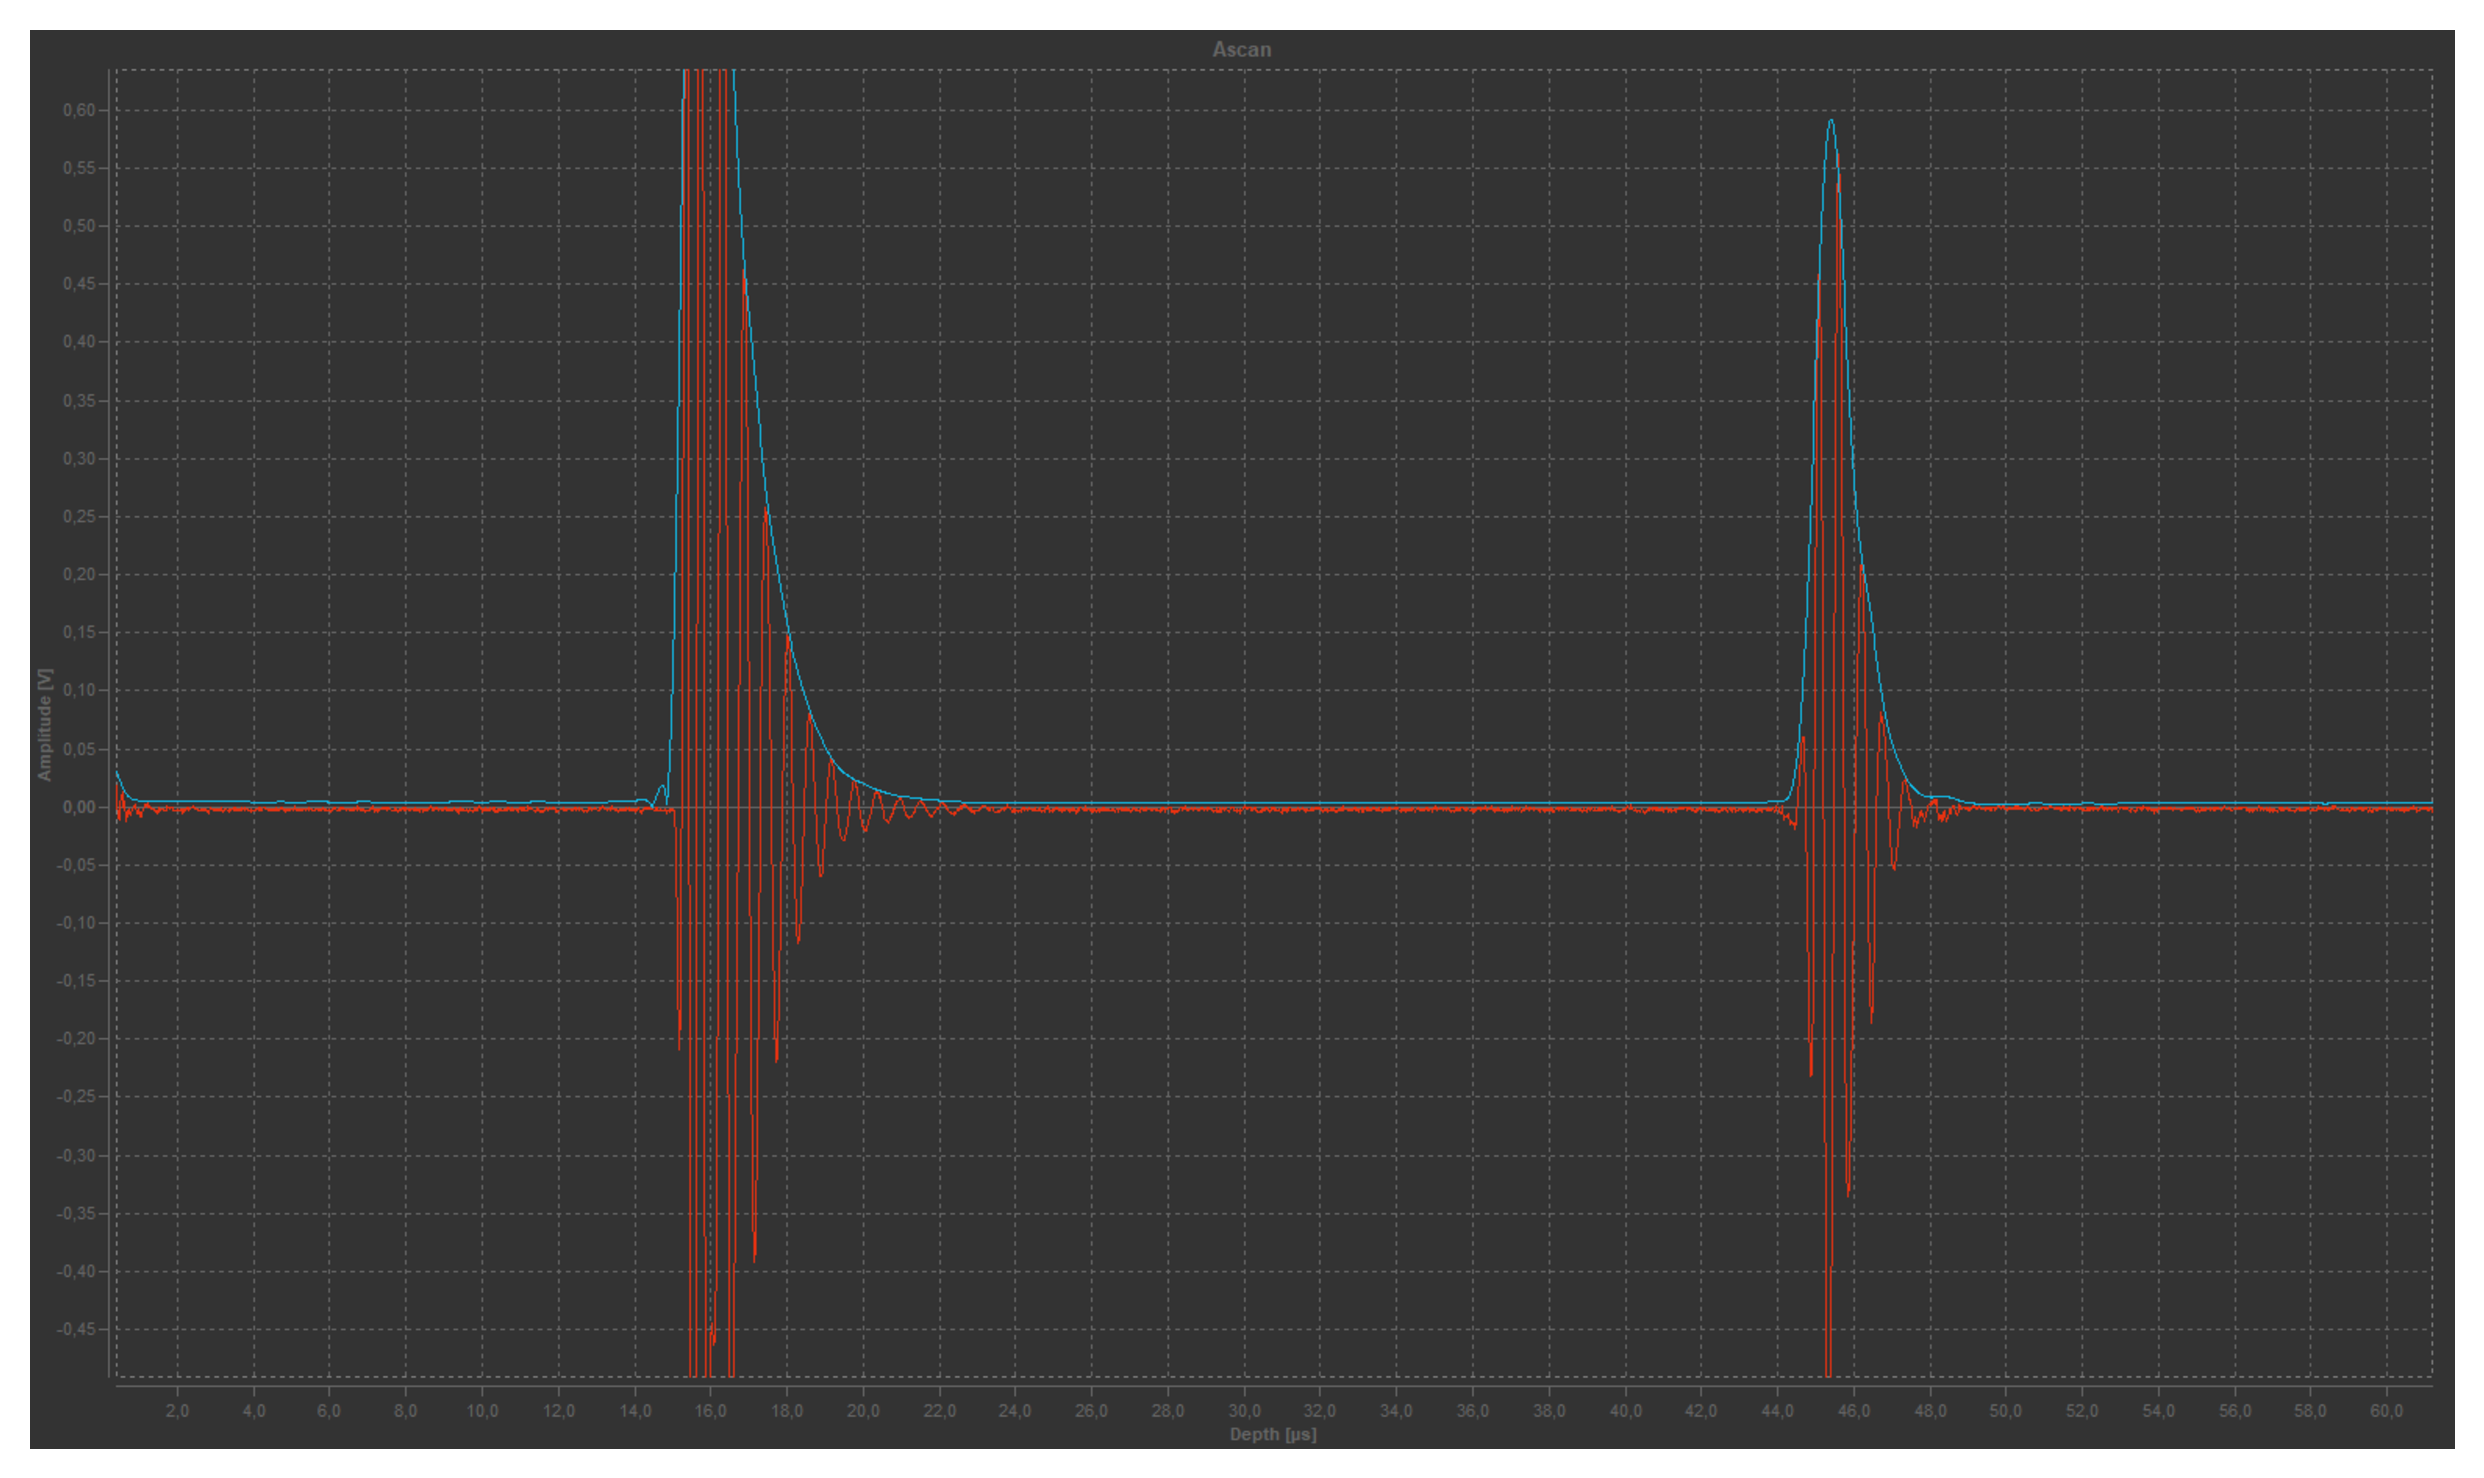
\includegraphics[width=\linewidth]{pictures/Durchschallung/z1.pdf}%
  \caption{Der erste Zylinder.}%
  \label{fig:durchschallung_z1}%
  \end{subfigure}%
  \hfill%
  \begin{subfigure}{0.48\textwidth}%
  \centering%
  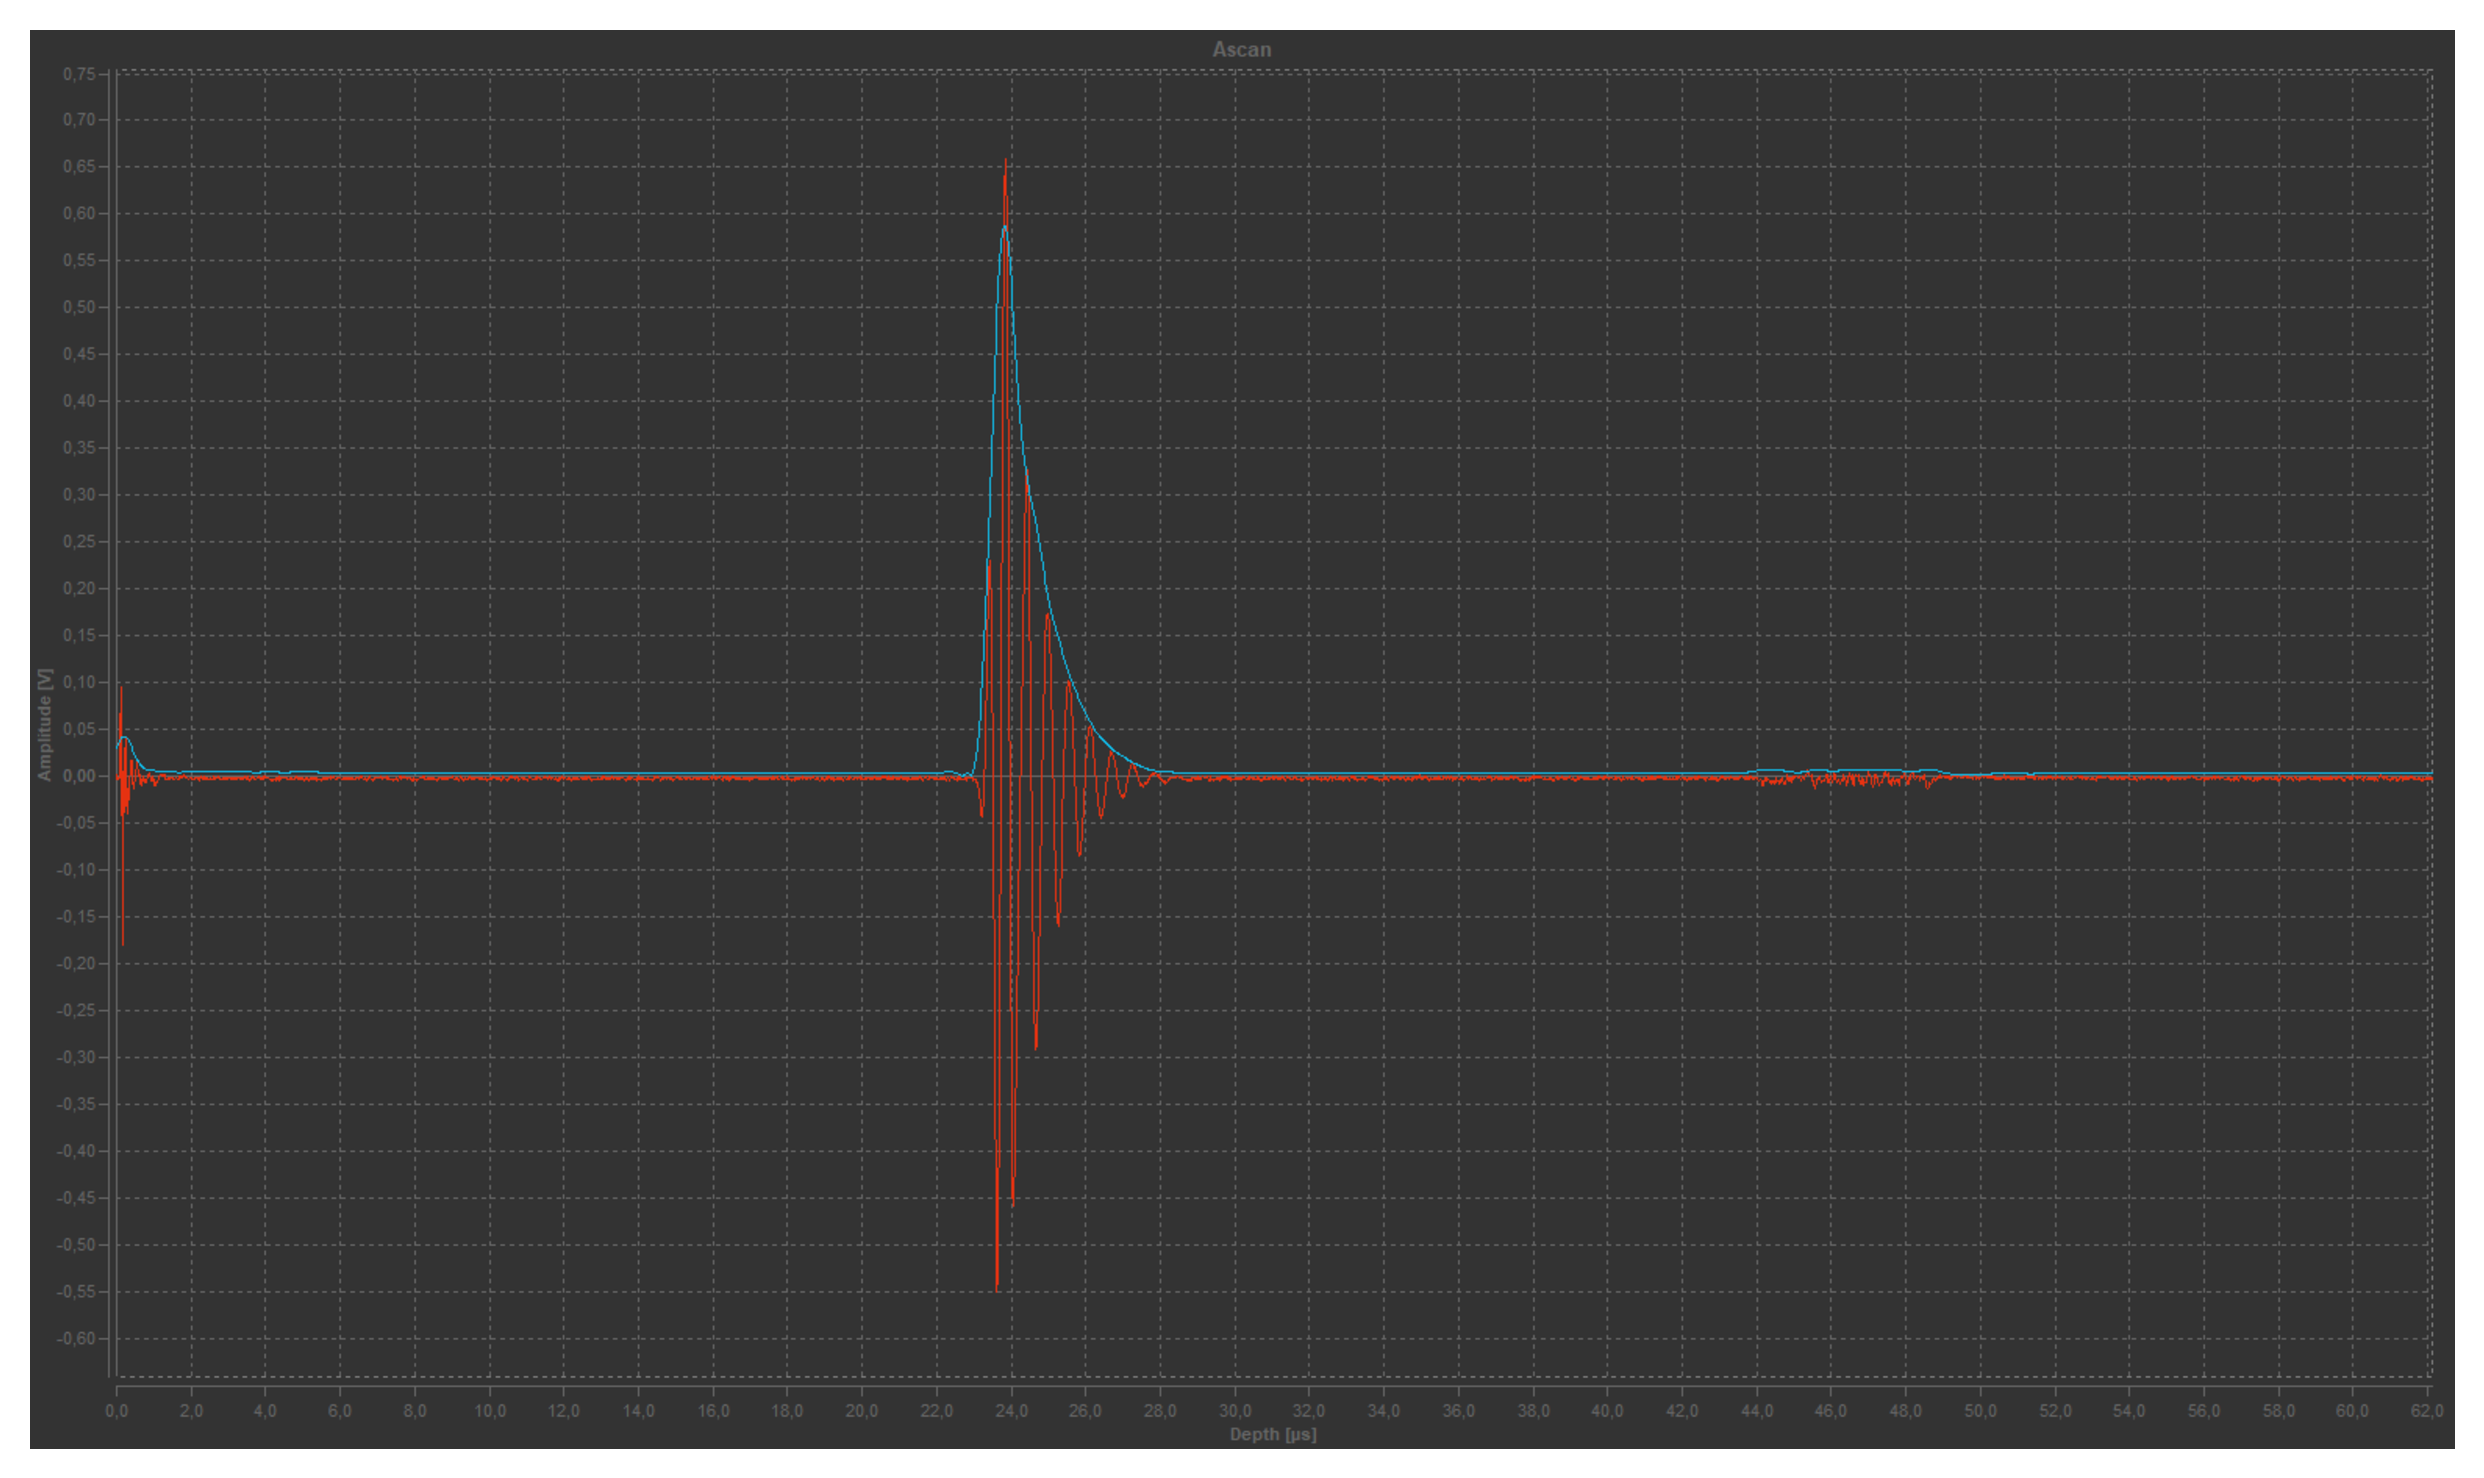
\includegraphics[width=\linewidth]{pictures/Durchschallung/z2.pdf}%
  \caption{Der zweite Zylinder.}%
  \label{fig:durchschallung_z2}%
  \end{subfigure}%
  \hfill

  \begin{subfigure}{0.48\textwidth}%
  \centering%
  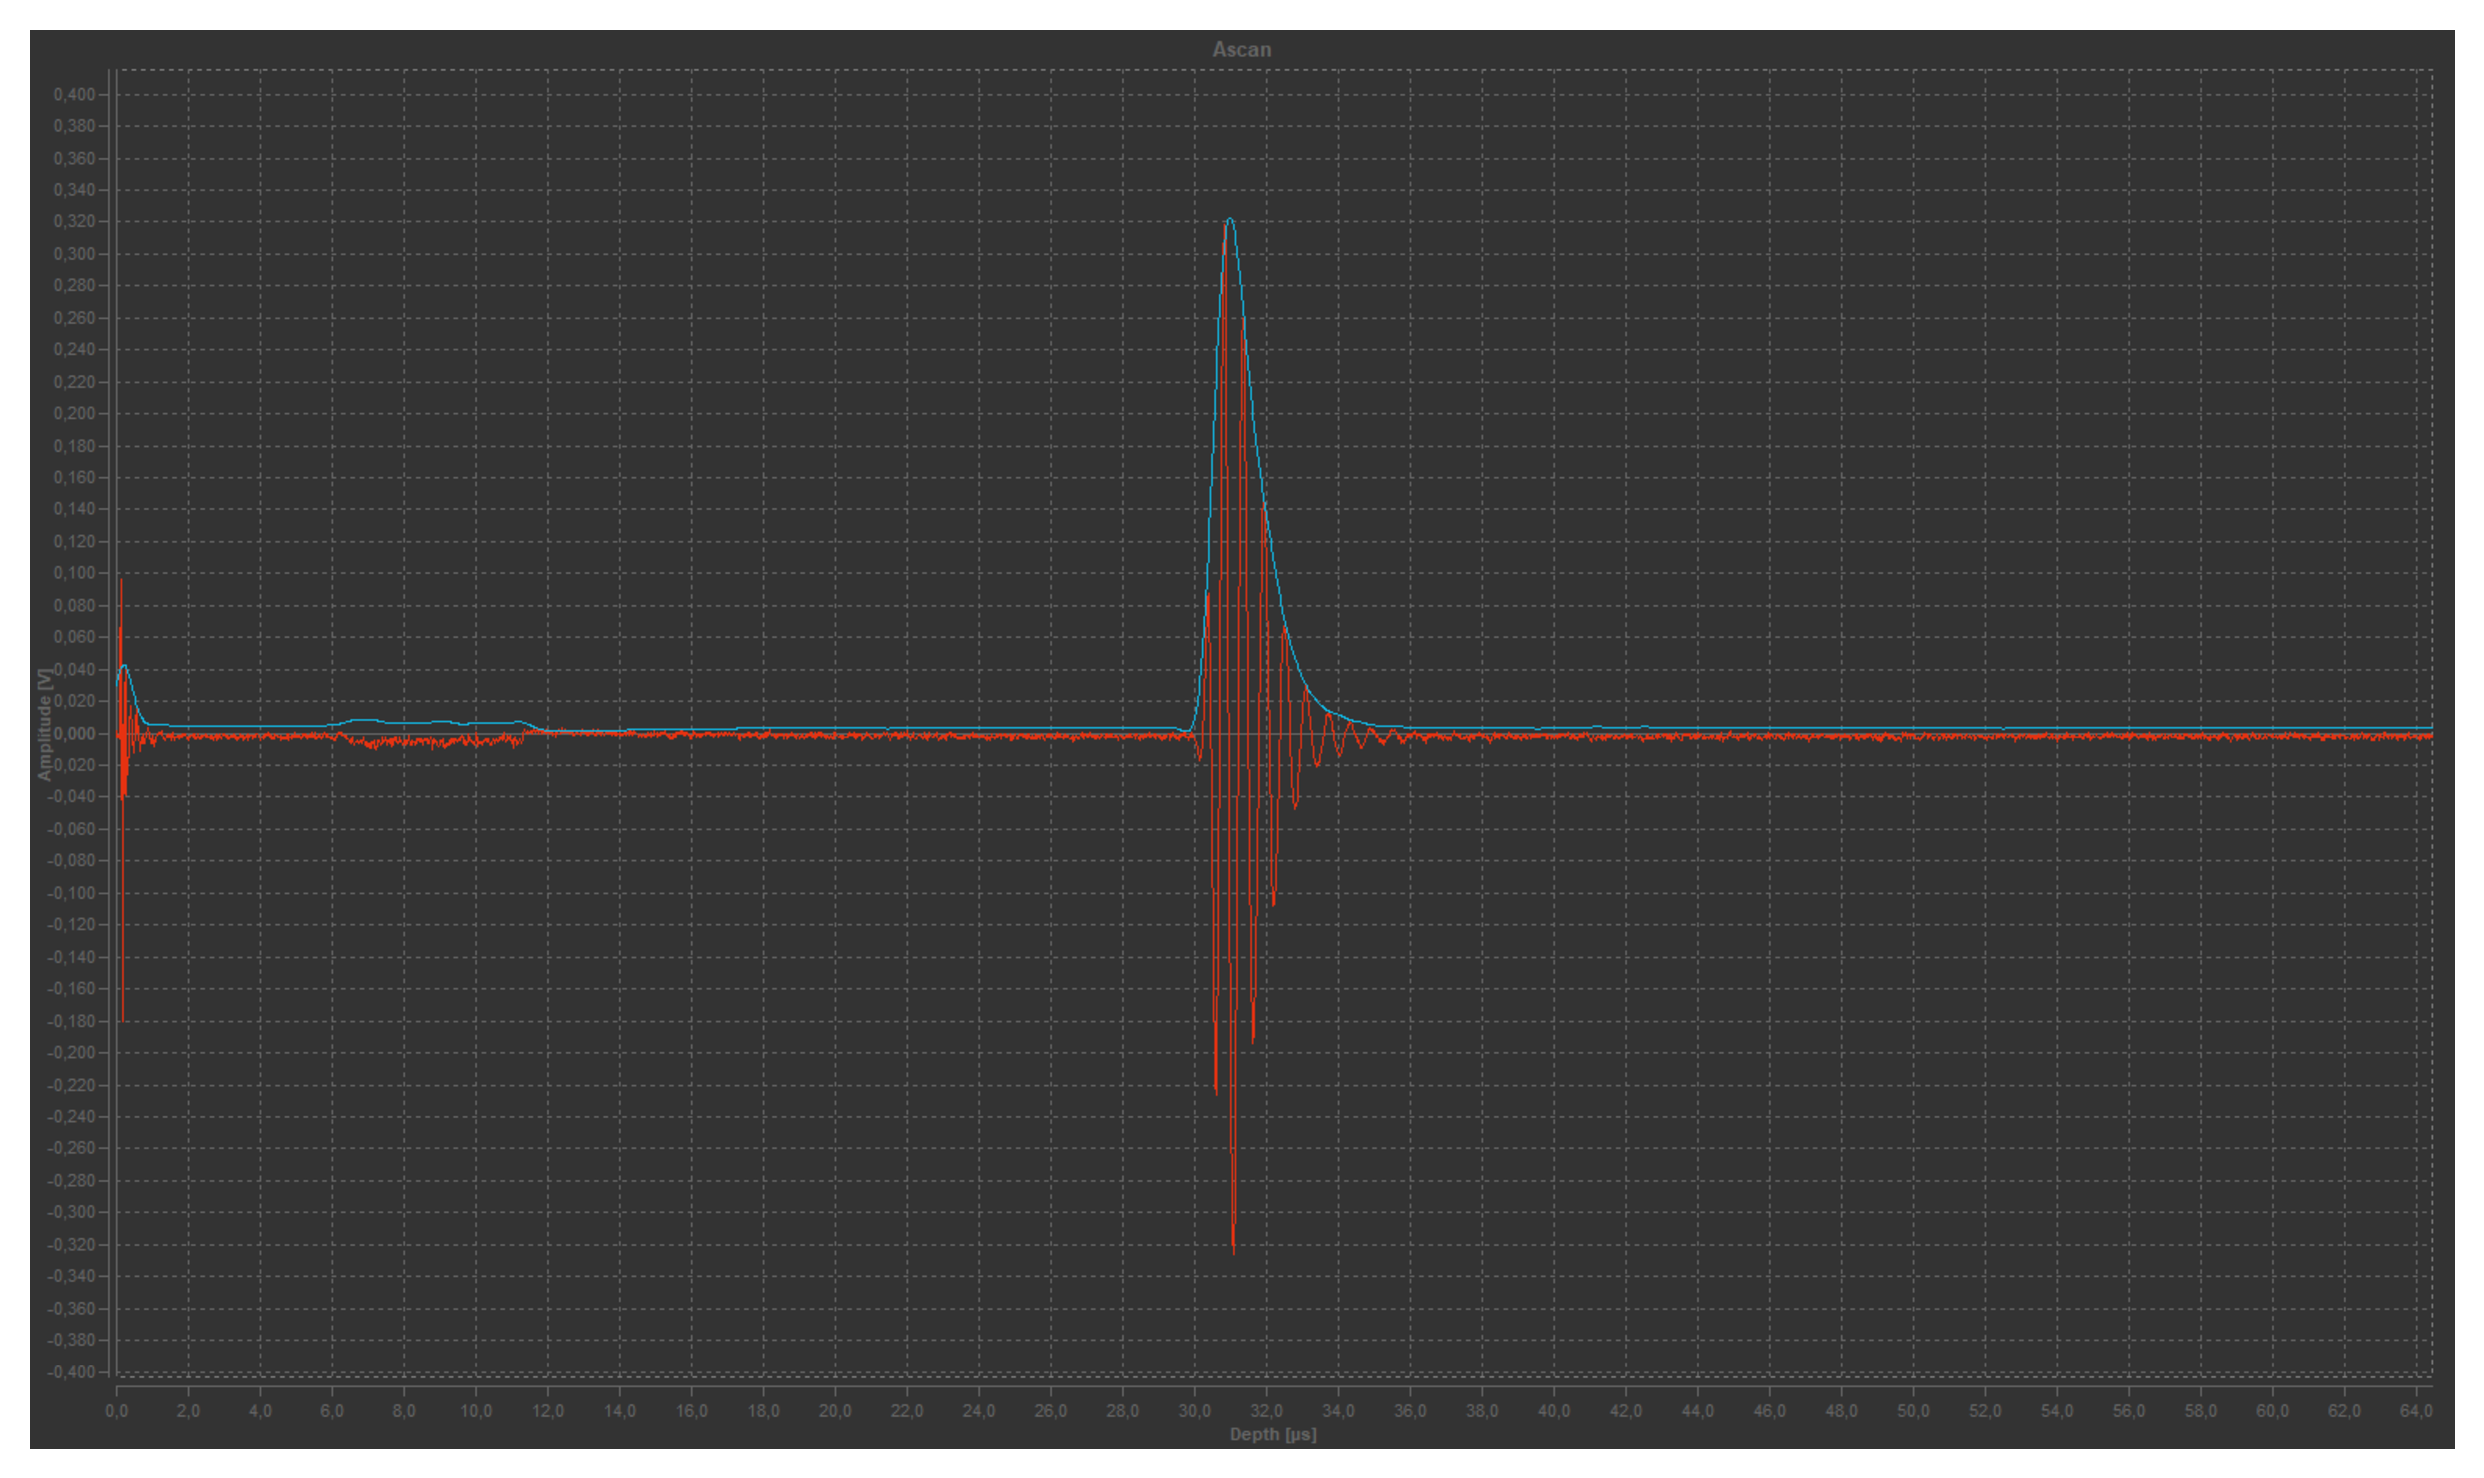
\includegraphics[width=\linewidth]{pictures/Durchschallung/z3.pdf}%
  \caption{Der dritte Zylinder.}%
  \label{fig:durchschallung_z3}%
  \end{subfigure}%
  \hfill%
  \begin{subfigure}{0.48\textwidth}%
  \centering%
  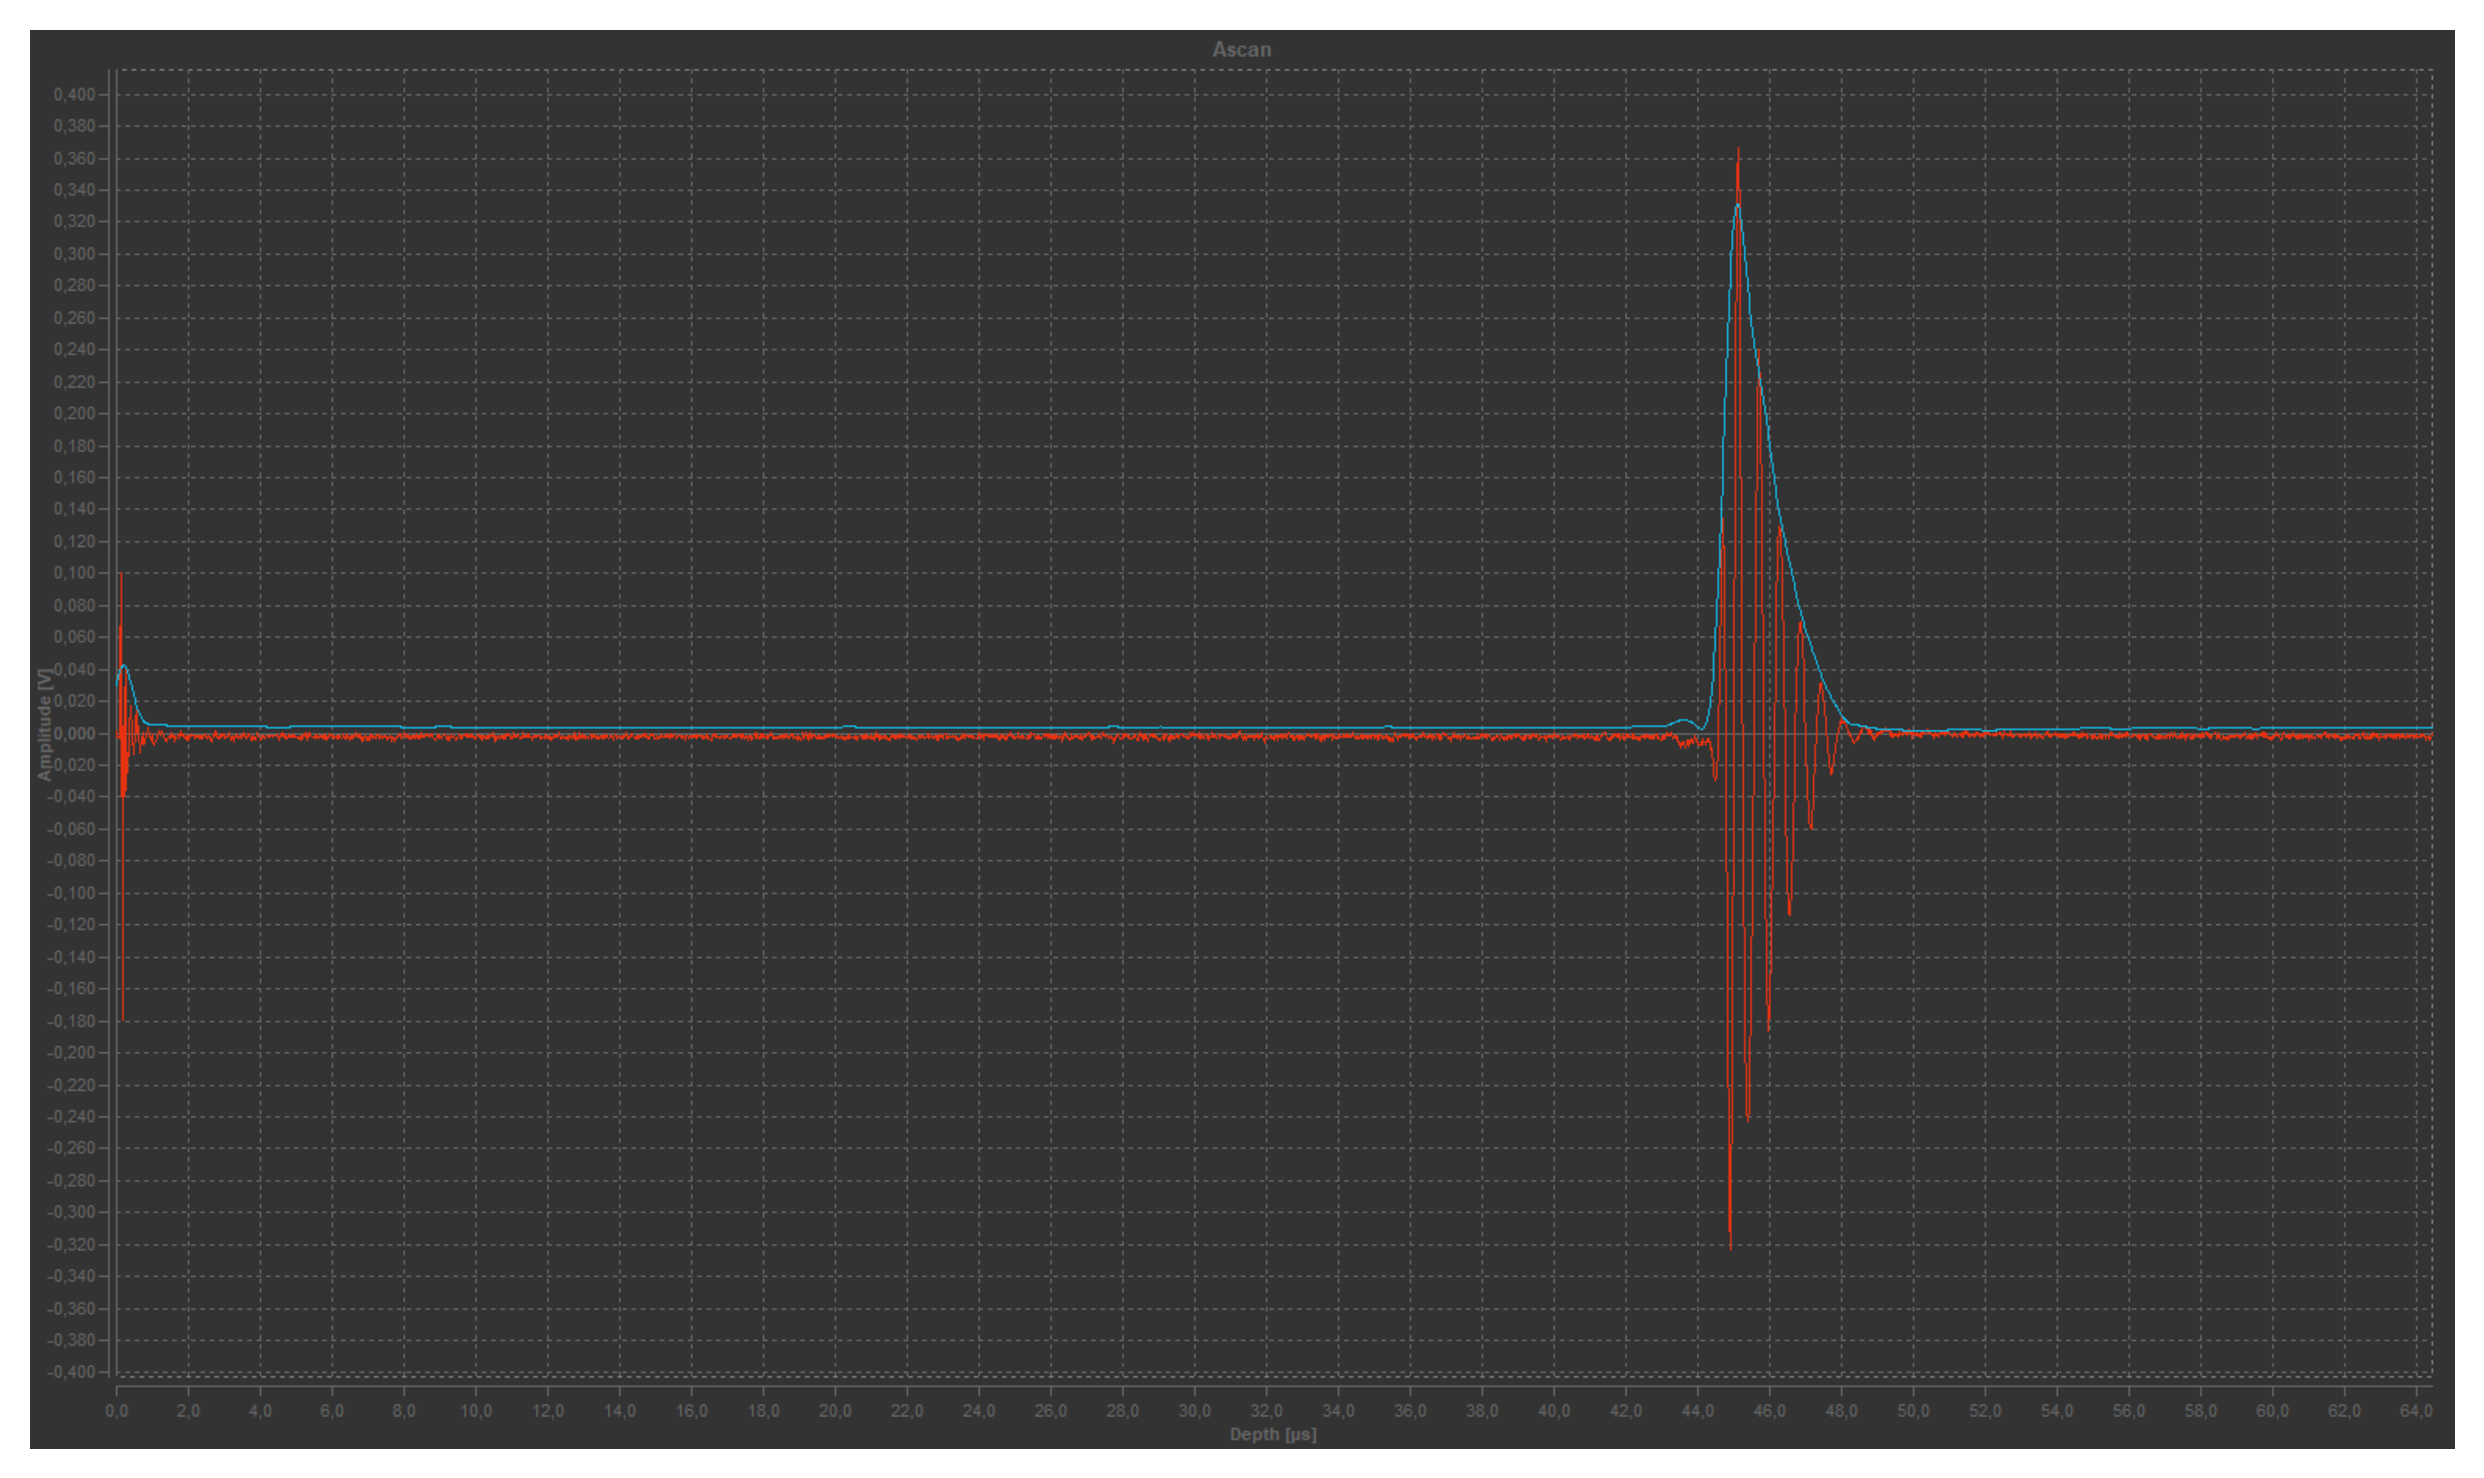
\includegraphics[width=\linewidth]{pictures/Durchschallung/z4.pdf}%
  \caption{Der vierte Zylinder.}%
  \label{fig:durchschallung_z4}%
  \end{subfigure}%
  \hfill
  \caption{Die Messungen des Durchschallungsverfahrens}%
  \label{fig:durchschallung_messungen}%
\end{figure}%


\subsection{Bestimmung der Dämpfung mit dem Impuls-Echo-Verfahren}

Als nächstes soll aus den Amplituden der Messung die Dämpfungskonstante $\alpha$ aus \autoref{eq:Intensität} bestimmt werden.
Dafür wird in der Gleichung $x = 2 \cdot d$ gewählt und für die lineare Regression wird die Gleichung logarithmiert.
Es ergibt sich der Ansatz
\begin{equation*}
  ln \left( \frac{I}{I_0} \right) = - \alpha \cdot 2 \cdot d \, .
\end{equation*}
Dafür werden die Messdaten der Amplitude in \autoref{tab:echo_messungen} verwendet.
Es ergibt sich
\begin{equation*}
  \alpha = 28.3 \pm 1.3 \, .
\end{equation*}
Die Regressionsgerade ist in \autoref{fig:plot3} dargestellt.

\begin{figure}
  \centering
  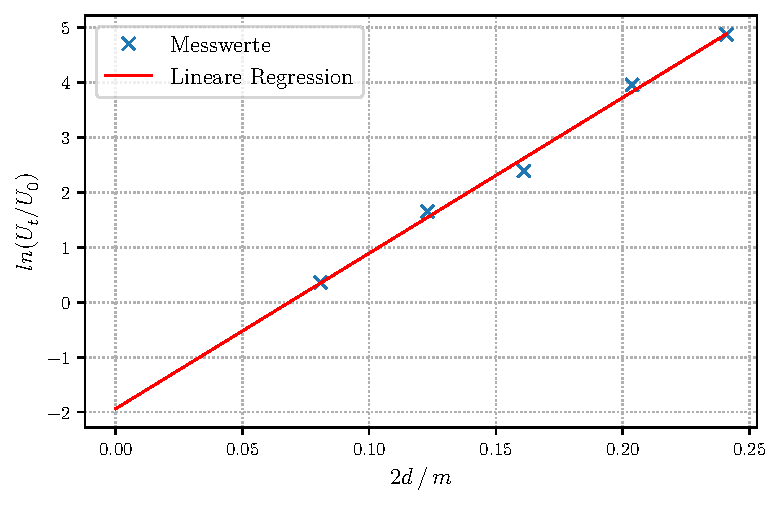
\includegraphics[width = 0.7\linewidth]{build/plot3.pdf}
  \caption{Regressionsgerade der Intensität in Abhängigkeit des Durchmessers.}
  \label{fig:plot3}
\end{figure}

\subsection{Vermessung des Augenmodells}

Die entsprechende Messung zu der Vermessung des Augenmodells ist in \autoref{fig:auge} dargestellt
und es sind fünf Peaks zu erkennen. Dabei ist der erste Peak (Peak 0) zu vernachlässigen.
Aus der Messung lassen sich dann die Messdaten in \autoref{tab:auge} ablesen.
Dabei werden die Peaks den folgenden Bestandteilen des Auges zugeordnet:
\begin{align*}
  \text{Peak 0} &\to \text{Hornhaut} \\
  \text{Peak 1} &\to \text{Anfang der Linse} \\
  \text{Peak 2} &\to \text{Ende der Linse} \\
  \text{Peak 3} &\to \text{Netzhaut} \\
  \text{Peak 4} &\to \text{Retina} \\  
\end{align*}
Mit den Schallgeschwindigkeiten $c_L = 2500 \unit{\meter / \second}$ und $c_{GK} = 1410 \unit{\meter / \second}$.
Aus der allgemeinen Formel \ref{eq:s} ergeben sich dann
\begin{align*}
  \text{Hornhaut bis Anfang der Linse}&: s_1 = \frac{1}{2} c_{GK} \cdot t_1 = 0.846 \, \unit{\centi\meter} \\
  \text{Hornhaut bis Ende der Linse}&: s_2 = \frac{1}{2} c_L \cdot (t_2 - t_1) + s_1 = 1.346 \, \unit{\centi\meter} \\
  \text{Hornhaut bis Netzhaut}&: s_3 = \frac{1}{2} c_{GK} \cdot (t_3 - t_2) + s_2 = 1.834 \, \unit{\centi\meter} \\
  \text{Hornhaut bis Retina}&: s_4 = \frac{1}{2} c_{L} \cdot (t_4 - t_3) + s_3 = 8.59 \, \unit{\centi\meter} 
\end{align*}


\begin{table}
  \centering
  \caption{Messdaten der Vermessung des Auges.}
  \label{tab:auge}
  \begin{tabular}{c c}
      \toprule
      Peak Nummer & t / \unit{\micro\second}\\ 
      \midrule
      1 & 12\\
      2 & 16\\
      3 & 23\\
      4 & 77\\
      \bottomrule
  \end{tabular}
\end{table}

\begin{figure}
  \centering
  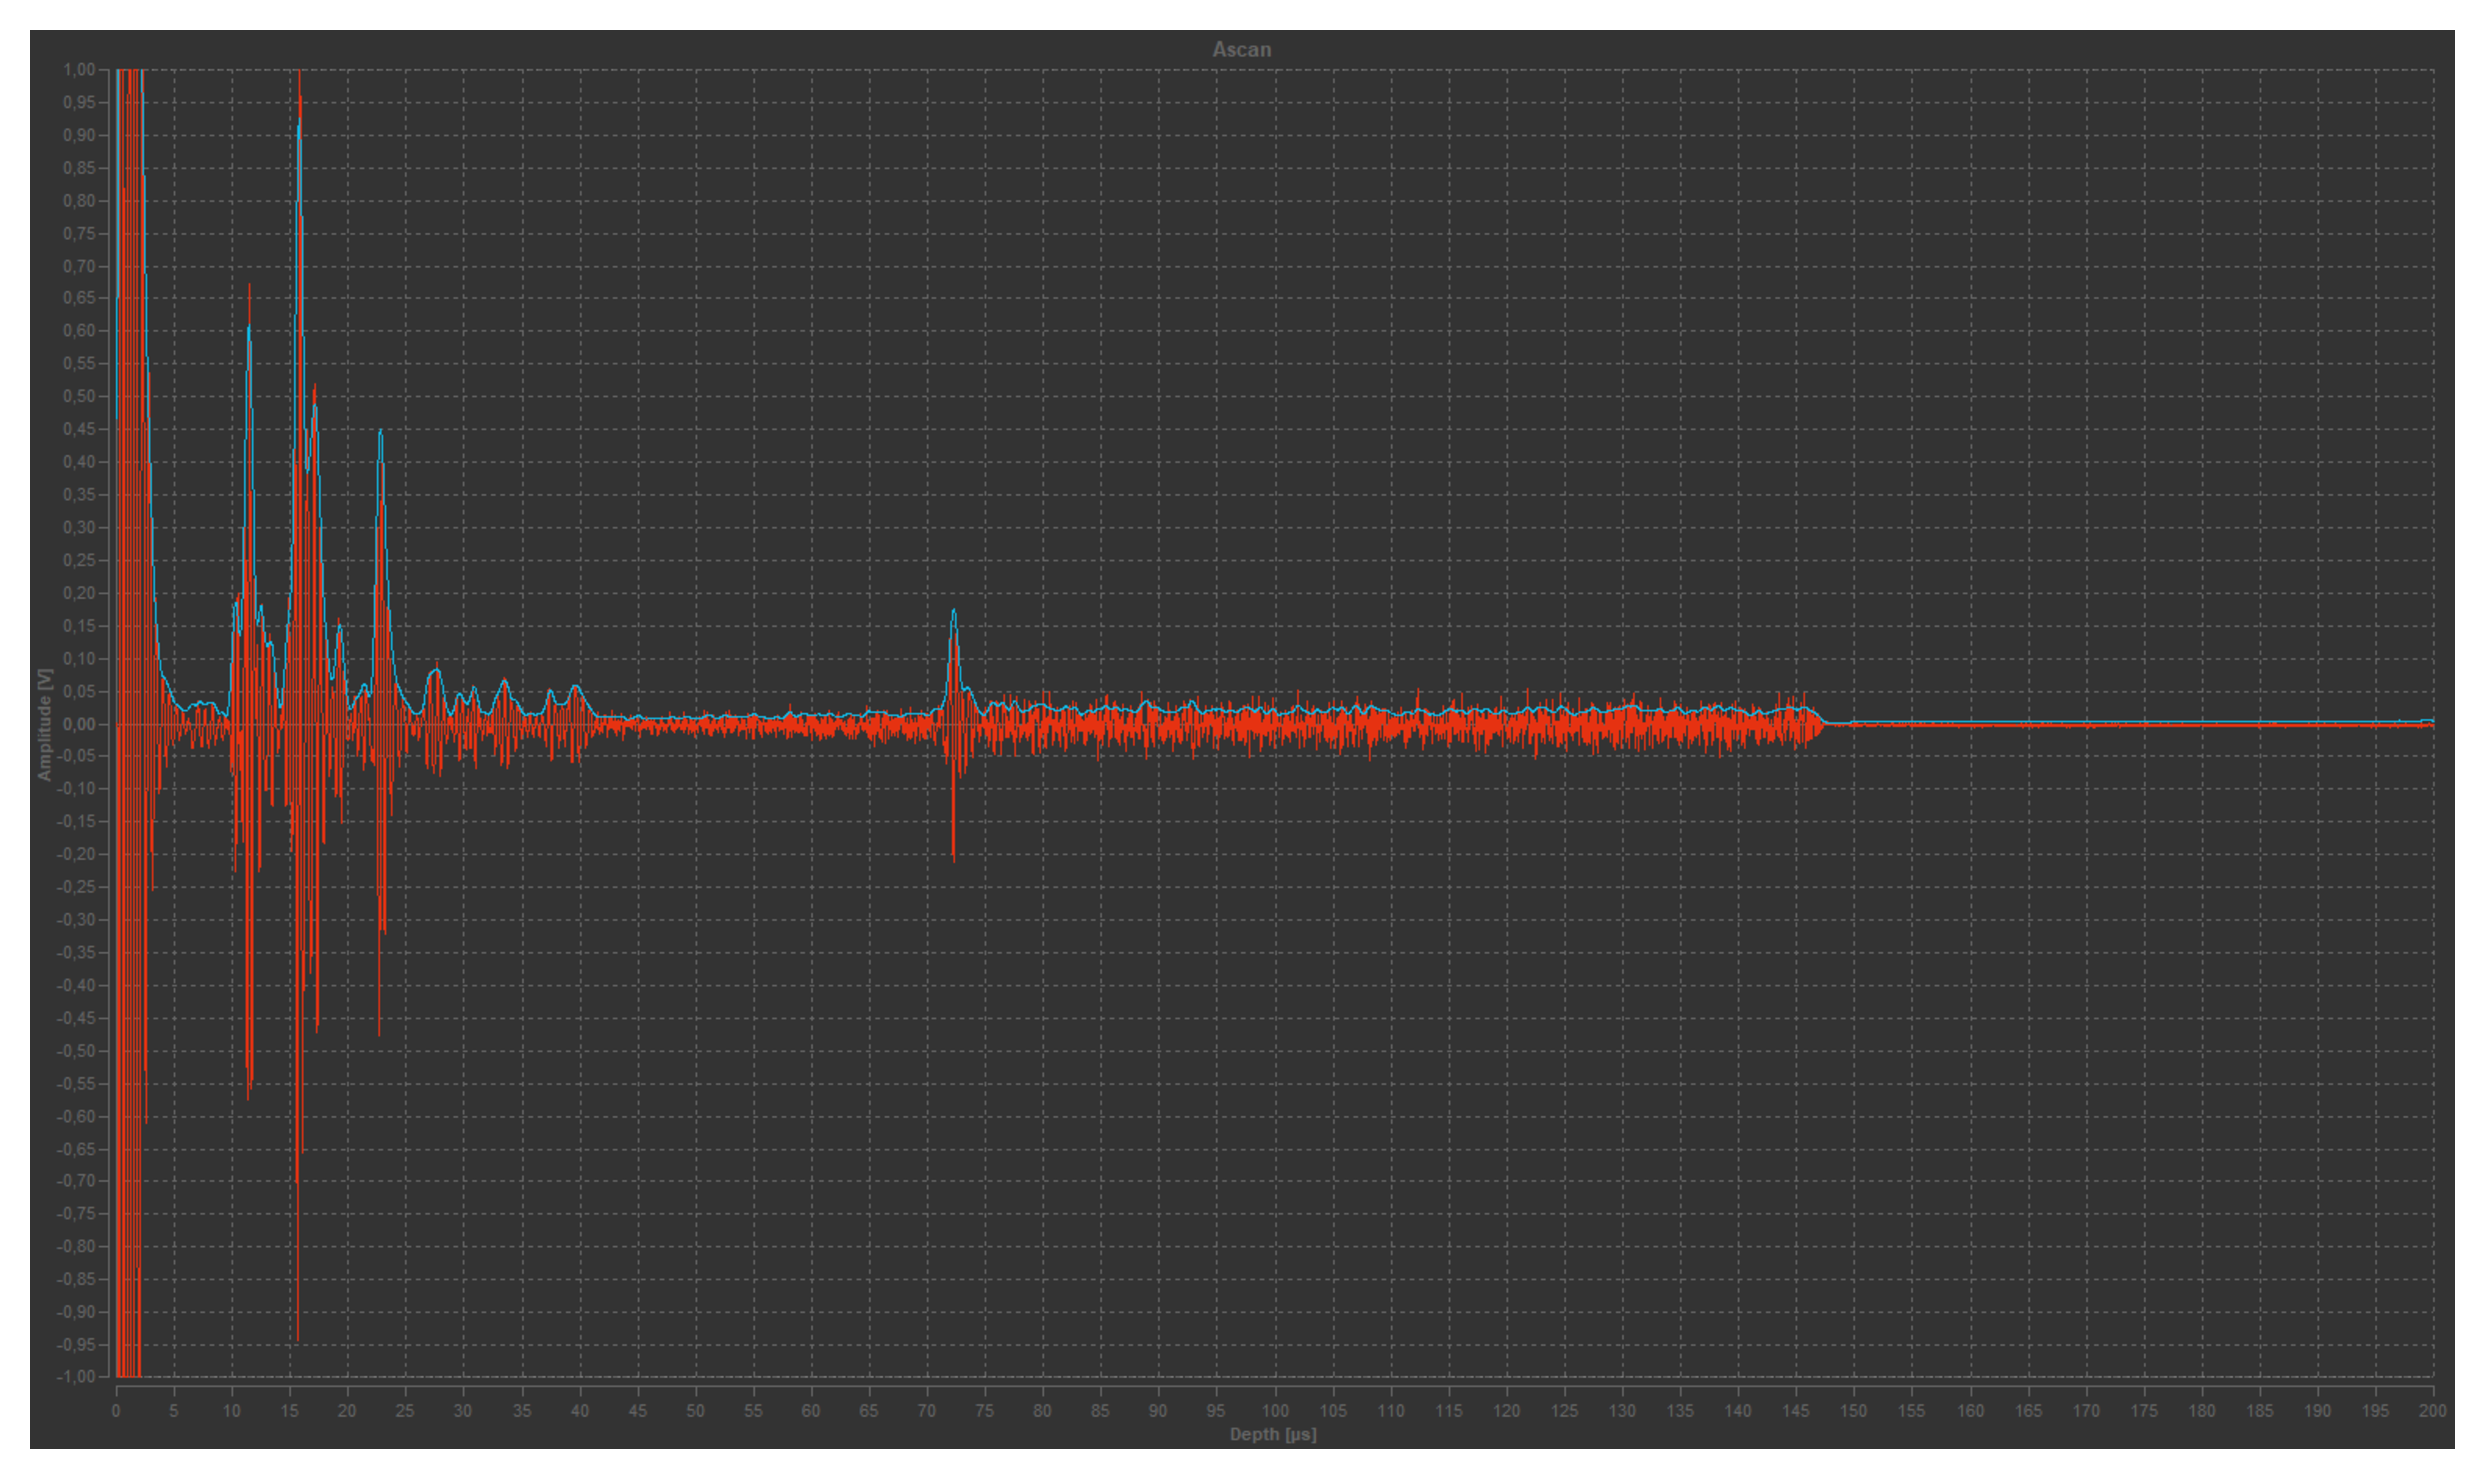
\includegraphics[width = 0.8\linewidth]{pictures/auge/Messung1Auge.pdf}
  \caption{Screenshot der Messung des Augenmodells}
  \label{fig:auge}
\end{figure}